
\clearpage

\section{Explorando PDB4DNA}
\label{sec:MODIFI}
\begin{figure}[htbp]
    \centering
    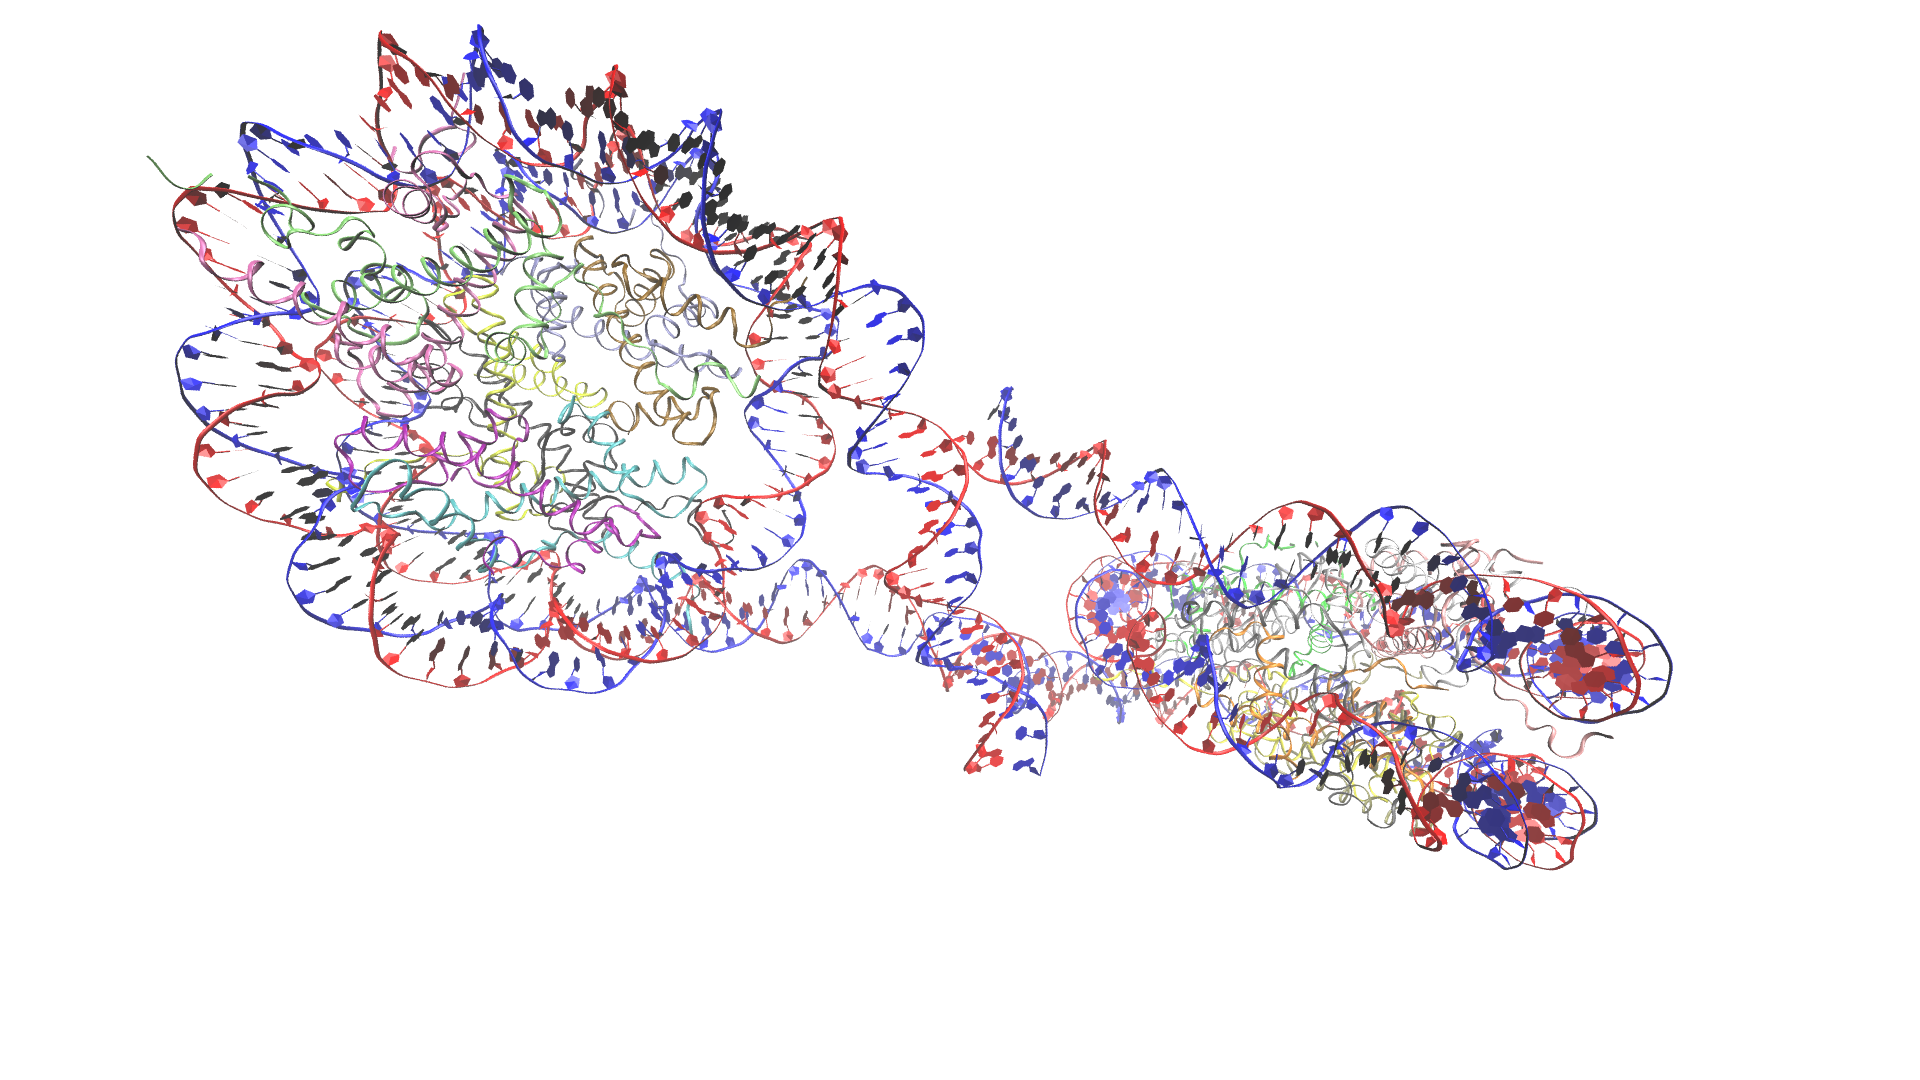
\includegraphics[width=0.8\linewidth]{./Figures/1ZBB.png}
    \caption[Molécula de ADN 1ZBB]{Molécula de ADN 1ZBB vista en VMD}
    \label{fig:1zbb}
\end{figure}

\begin{figure}[htbp]
    \centering
    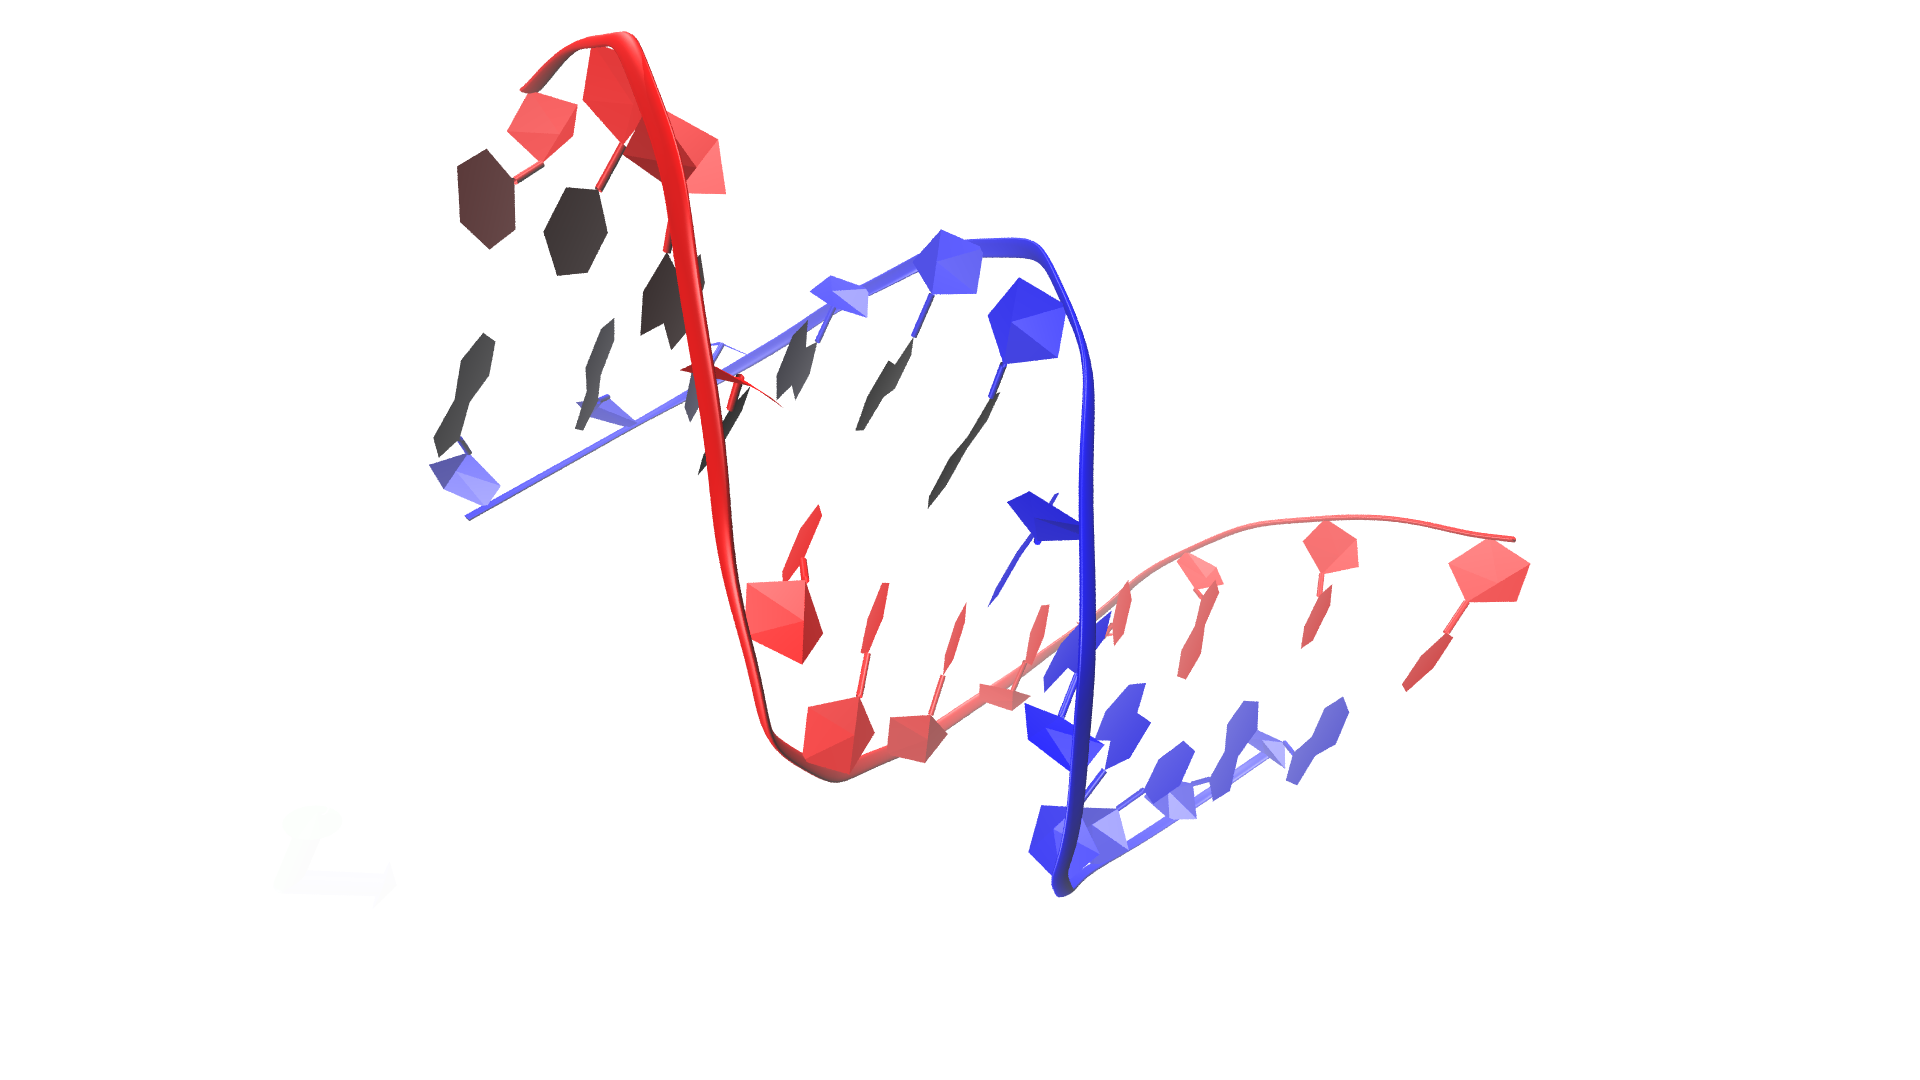
\includegraphics[width=0.8\linewidth]{./Figures/1FZX.png}
    \caption[Molécula de ADN 1FZX]{Molécula de ADN 1FZX vista en VMD}
    \label{fig:1fzx}
\end{figure}
Con tal de entender el código de pdb4dna, sus alcances, y resultados, se hace necesario el explorarlo, para esto se hizo uso de dos diferentes moléculas de ADN, 1ZBB(véase figura ~\ref{fig:1zbb} ) y 1FZX(véase figura ~\ref{fig:1fzx}), Se generaron histogramas de deposición de energía junto con los rompimientos simples y dobles, estos se realizaron con 10000 eventos con diferentes valores de energía para un electrón y un baryon con nombres en Geant4 e- y proton respectivamente, véase figuras ~\ref{fig:e}, ~\ref{fig:p}, ~\ref{fig:e2}, ~\ref{fig:p2}, de estos histogramas es interesante notar como los rompimientos simples y doble aumentan hasta cierto valor y luego empiezan a reducirse, esto puede deberse a diversos factores como el tamaño de la molécula y en cuantos enlaces se puede depositar la energía, también es necesario mencionar que en el stepping action la energía y las posiciones donde se deposita la energía se obtiene mediante la librería step y para ser precisos con la siguiente linea de código:
\lstset {language=C++}
\begin{lstlisting}
// Get position and edep of current step
    //
    G4double x = theStep->GetPreStepPoint()->GetPosition().x()/nanometer;
    G4double y = theStep->GetPreStepPoint()->GetPosition().y()/nanometer;
    G4double z = theStep->GetPreStepPoint()->GetPosition().z()/nanometer;
G4double edepStep = theStep->GetTotalEnergyDeposit()/eV;
\end{lstlisting}

Al graficar los baricentros de 1ZBB contra estas deposiciones de la energía debido a la partícula(figura ~\ref{fig:edep}) se puede ver en que partes se esta depositando la energía para cierto evento con ciertas condiciones, nótese que  bien lo que hace el código es filtrar la energía para que el programa genere un histograma de deposición de energía en donde solo se deposito energía en el fosfato o el azúcar , esto lo hace mediante varias lineas de código, primero PDBlic se encarga de leer el pdb y luego de la división de base fosfato y azúcar, mediante el código:

\lstset {language=C++}
\begin{lstlisting}
if(residueListTemp->fResSeq == 1)
            {
              if(iii == 0) BSP = 0; //"Phosphate"
              else if(iii < 8) BSP = 1; //"Sugar"
              else BSP = 2; //"Base"
            }
            else
            {
              if(iii < 4) BSP = 0; //"Phosphate"
              else if(iii < 11) BSP = 1; //"Sugar"
              else BSP = 2; //"Base"
            }
\end{lstlisting}
Mediante esto se le da un valor numérico al fosfato 0, al azúcar 1 y a la base 0, luego en el stepping action si se encuentra un golpe ya sea en el azúcar o en el fosfato se retorna ese valor de energía, esto se hace mediante:
\lstset {language=C++}
\begin{lstlisting}
int numStrand=0;
  int numNucl=0;
  int intResidue=-1; // 0 for Phospat, 1 for Sugar, 2 for Base
  unsigned short int hit = (fpDetector->GetPDBlib()).ComputeMatchEdepDNA(
      fpDetector->GetBarycenterList(),
      fpDetector->GetMoleculeList(),
      x*10., y*10., z*10.,// x10 => angstrom<->nm
      numStrand, numNucl, intResidue);

  if (hit==1)
  {
    if ((intResidue==0)||(intResidue==1)) //Edep in Phosphate or Sugar
    {
      fpEventAction->AddEdepToNucleotide(numStrand,numNucl,edepStep);
      return true;
    }
    else
    {
      return false;
    }
    \end{lstlisting}

    De modificarse lo anterior reemplazando por intResidue=2 se puede analizar deposición de energía en las bases, además de esto se podría hallar una forma de recolectar datos sobre donde se realizaron los rompimientos y con ello se podría hacer uso de gromacs para estudiar la dinámica estructural de la molécula de ADN luego de la radiación realizada por Geant4, pero debido a que no tenemos noción de como se evaluá el daño por radiación en bases y por cuestiones de tiempo, esto no se llevara acabo por el momento.\\



\begin{figure}
\centering
\begin{subfigure}{.5\textwidth}
  \centering
  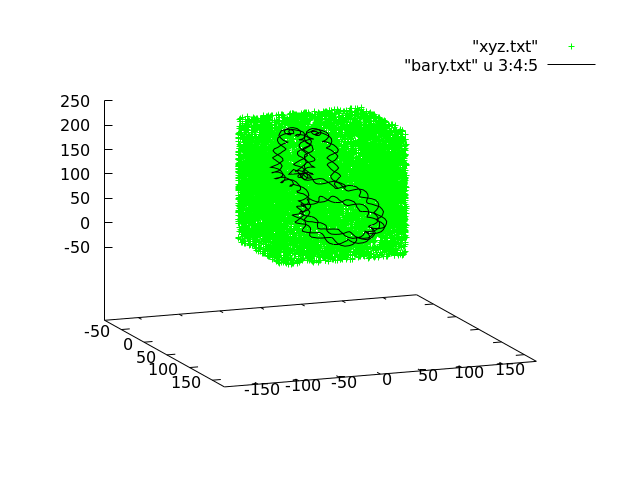
\includegraphics[width=1\linewidth]{./Figures/dep.png}
  \caption{Vista lateral}
  \label{fig:subeio1}
\end{subfigure}%
\begin{subfigure}{.5\textwidth}
  \centering
  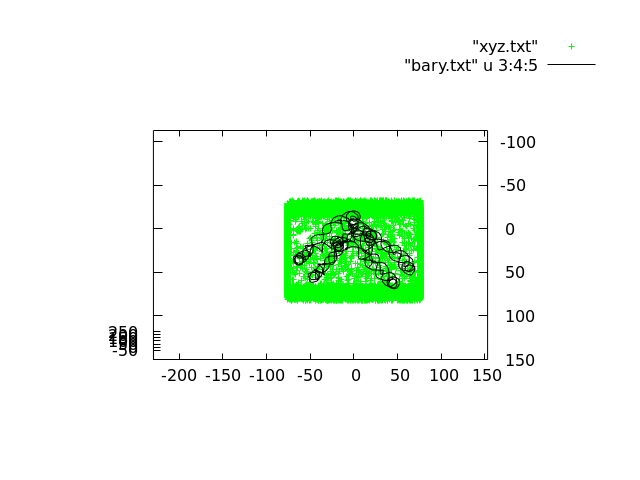
\includegraphics[width=1\linewidth]{./Figures/dep1.png}
  \caption{Vista superior}
  \label{fig:subeio2}
\end{subfigure}
\caption[Puntos de deposición de energía 1ZBB]{Puntos donde la partícula deposita energía en verde, y baricentros de 1ZBB en negro.}
\label{fig:edep}
\end{figure}




\begin{figure}
\centering
\begin{subfigure}{.5\textwidth}
  \centering
  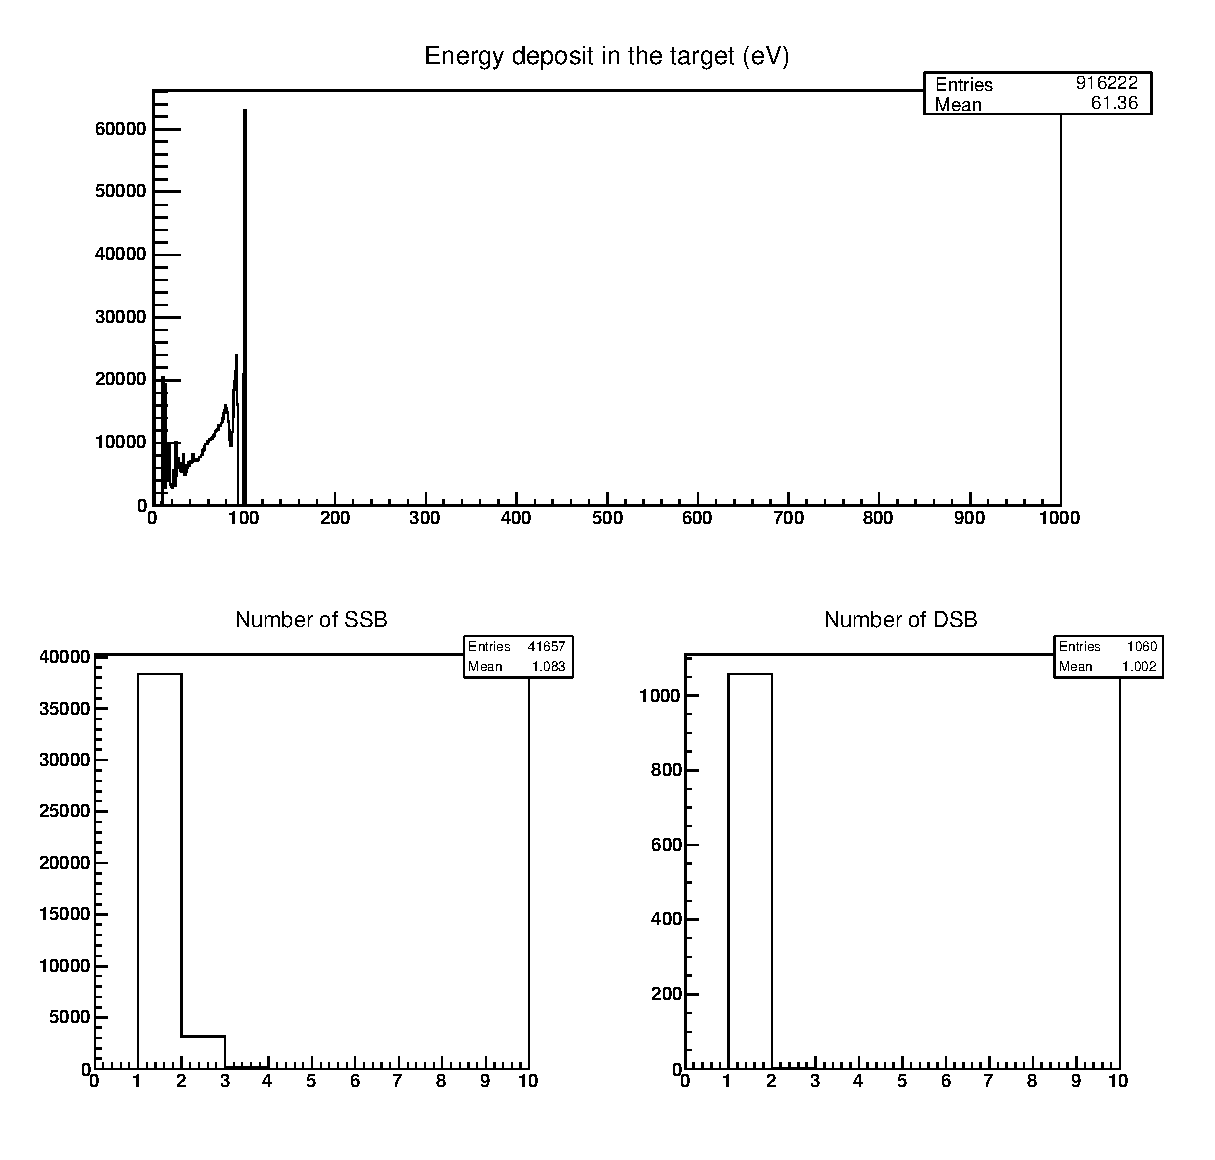
\includegraphics[width=.78\linewidth]{./Figures/1zbbe100ev.eps}
  \caption{100 eV}
  \label{fig:subei1}
\end{subfigure}%
\begin{subfigure}{.5\textwidth}
  \centering
  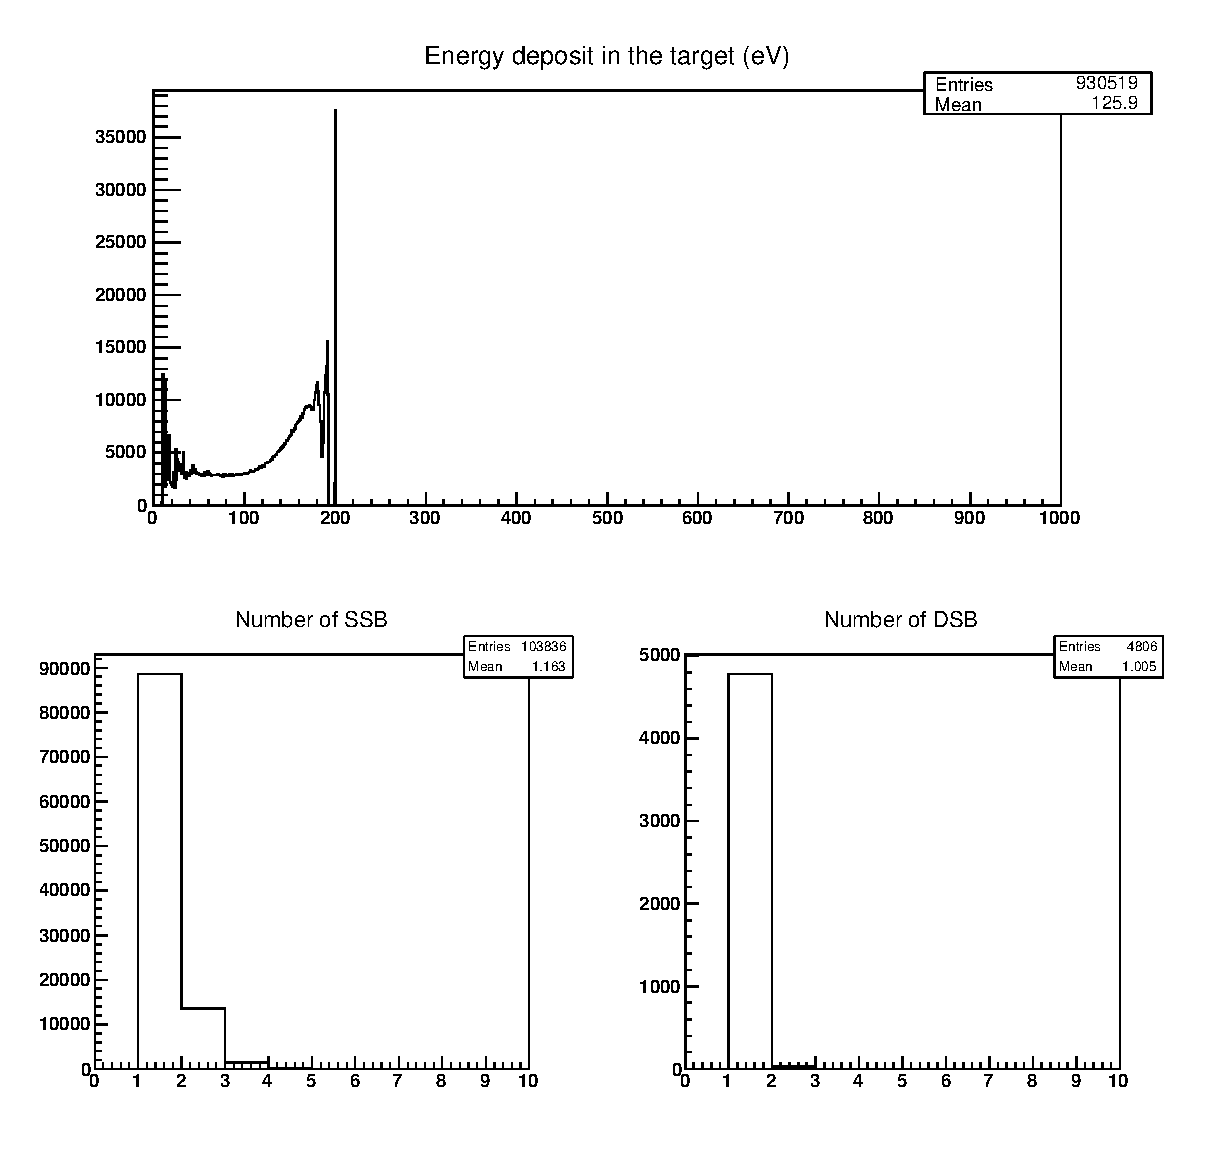
\includegraphics[width=.78\linewidth]{./Figures/1zbbe200ev.eps}
  \caption{200 eV}
  \label{fig:subei2}
\end{subfigure}
\begin{subfigure}{.5\textwidth}
  \centering
  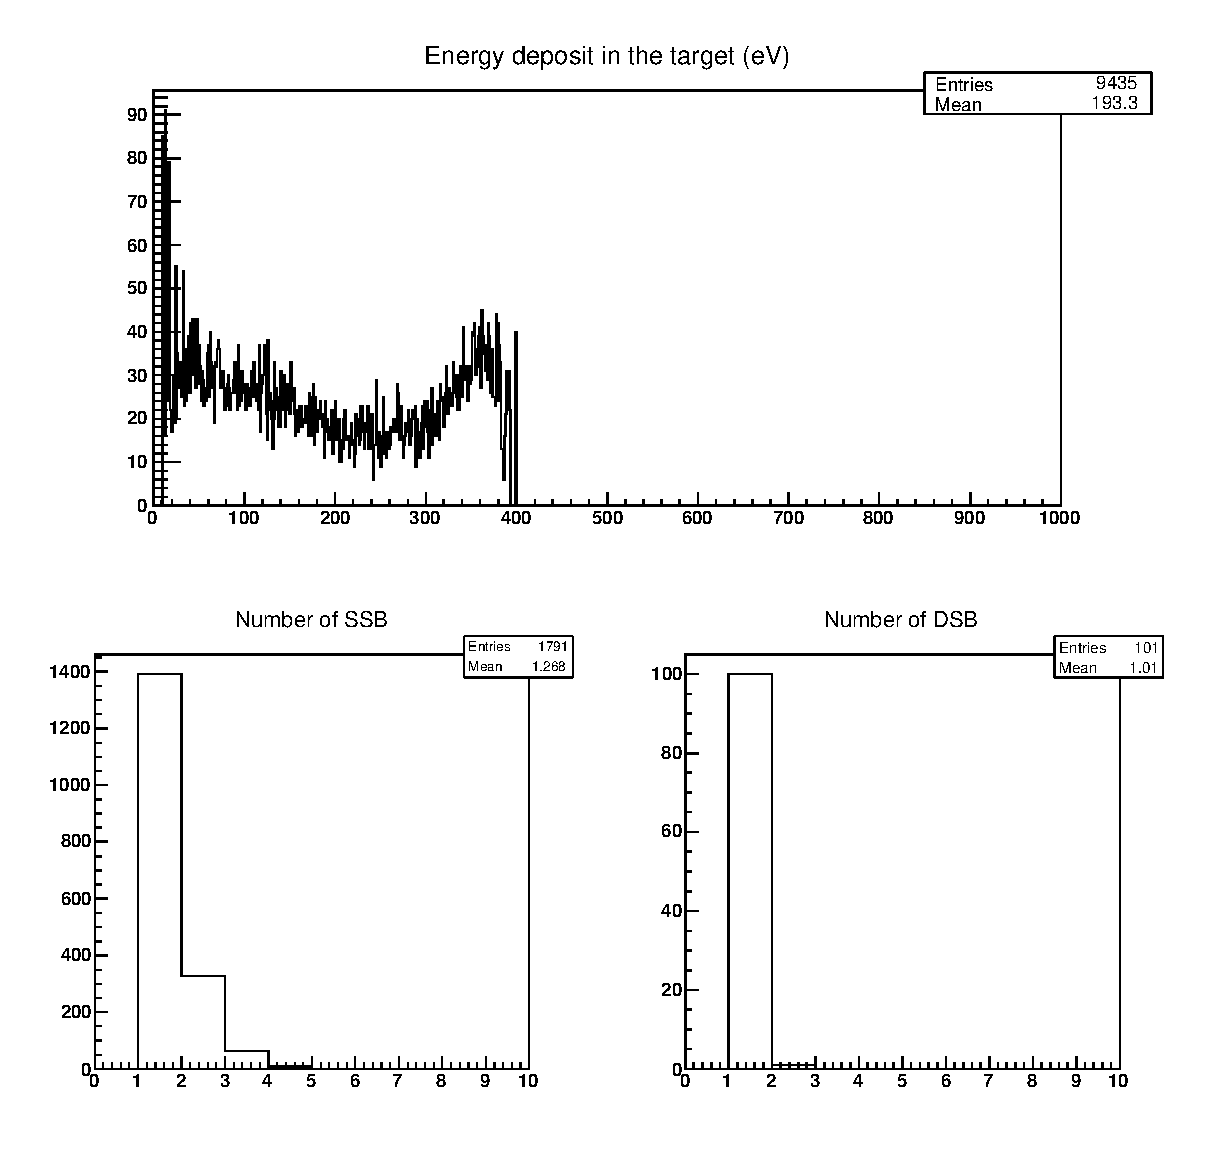
\includegraphics[width=.78\linewidth]{./Figures/1zbbe400ev.eps}
  \caption{400 eV}
  \label{fig:subei3}
\end{subfigure}%
\begin{subfigure}{.5\textwidth}
  \centering
  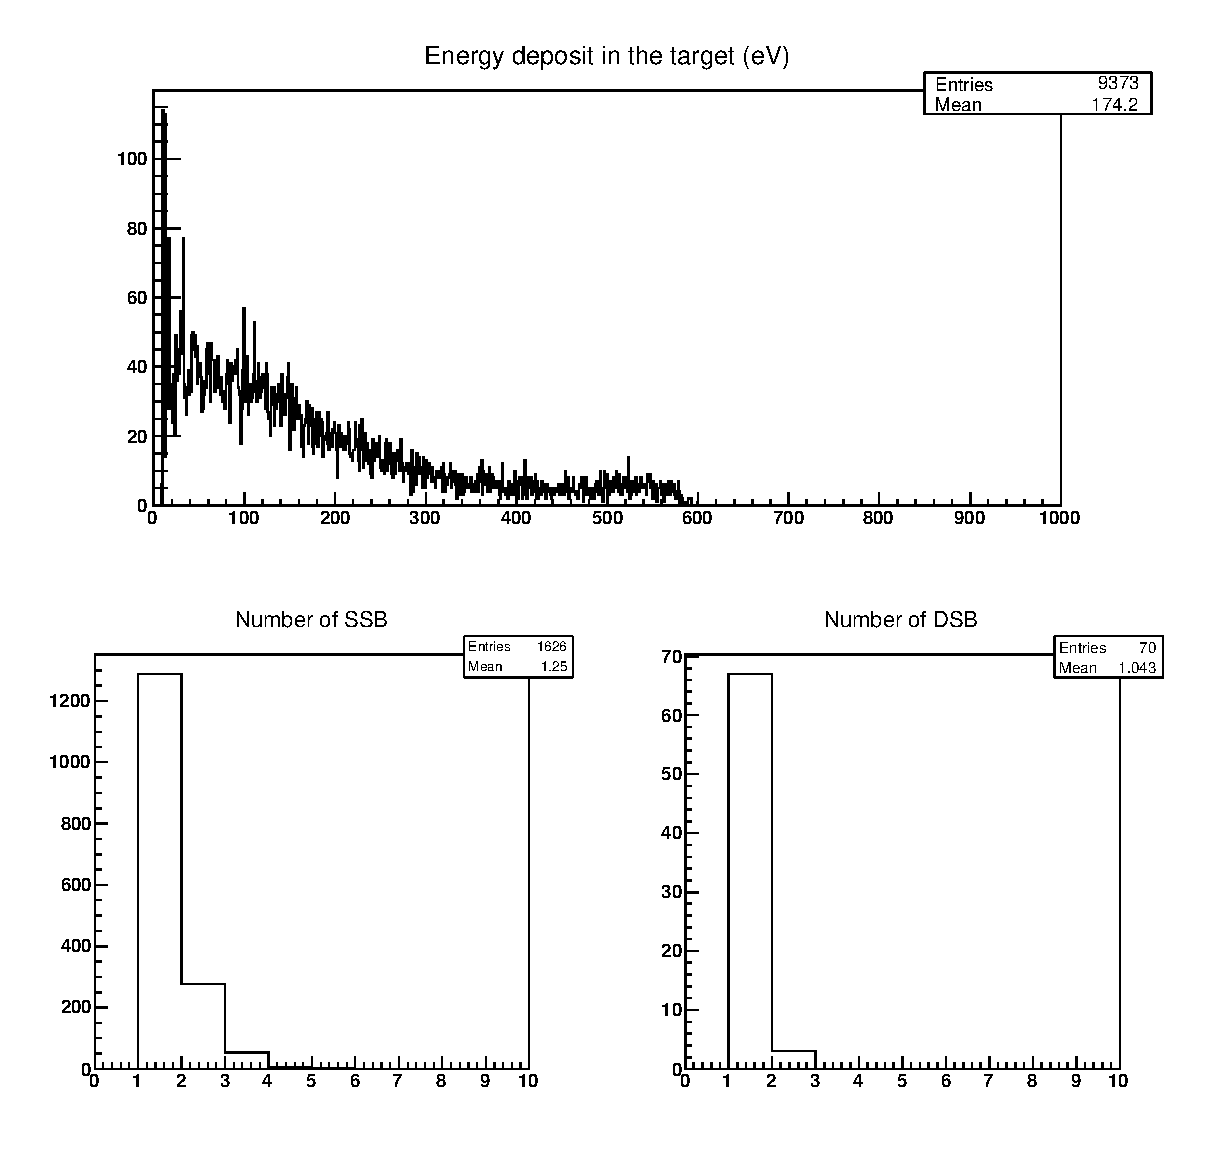
\includegraphics[width=.78\linewidth]{./Figures/1zbbe600ev.eps}
  \caption{600 eV}
  \label{fig:subei4}
\end{subfigure}
\begin{subfigure}{.5\textwidth}
  \centering
  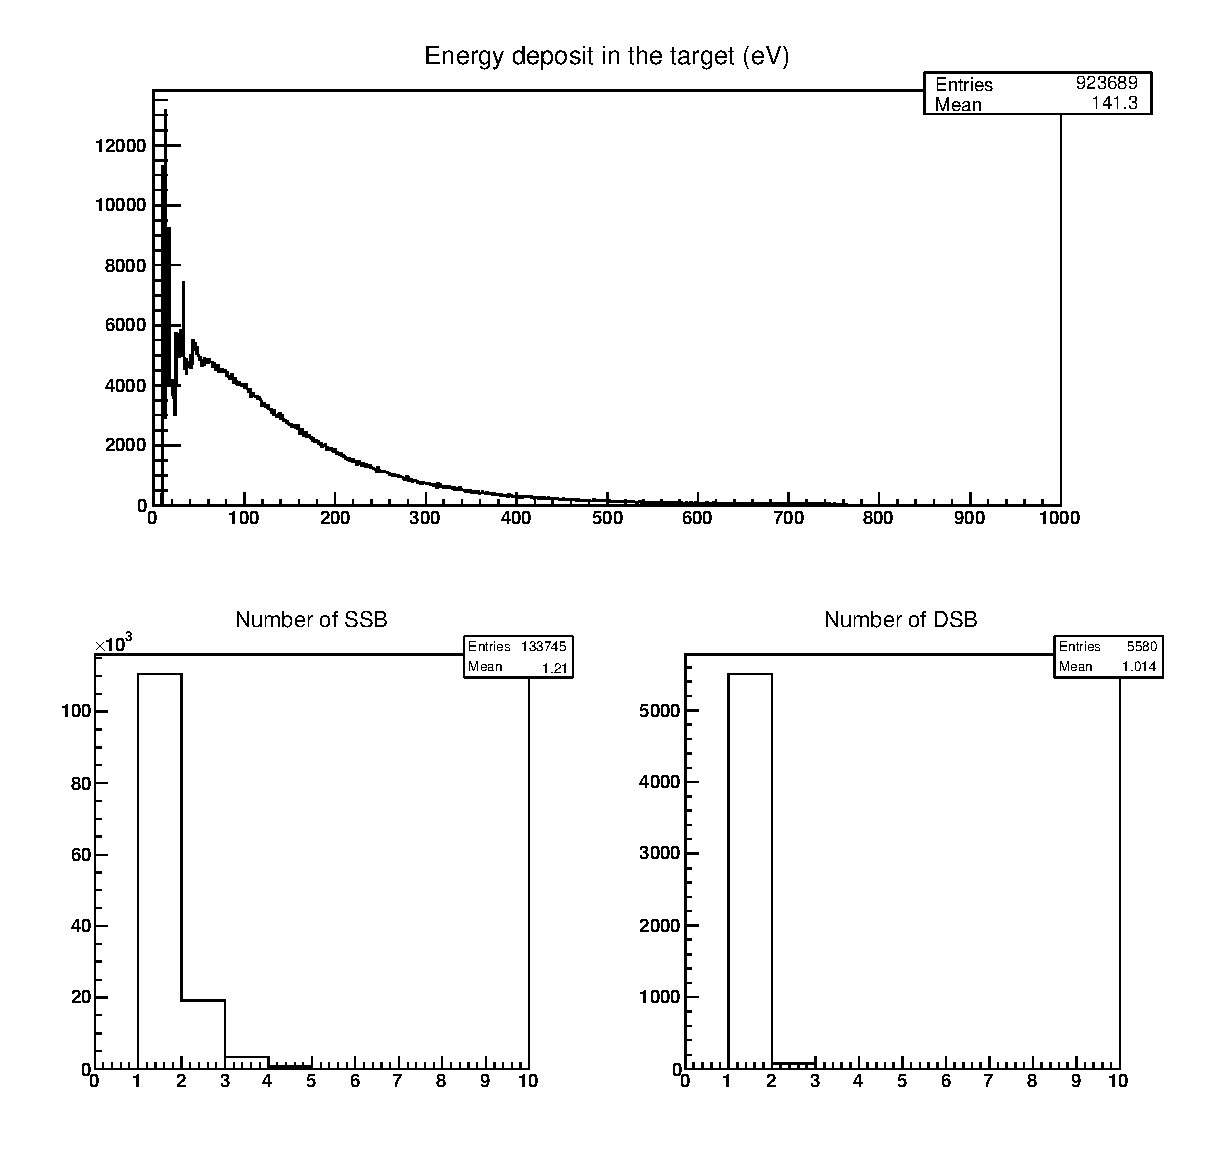
\includegraphics[width=.78\linewidth]{./Figures/1zbbe800ev.eps}
  \caption{800 eV}
  \label{fig:subei5}
\end{subfigure}%
\begin{subfigure}{.5\textwidth}
  \centering
  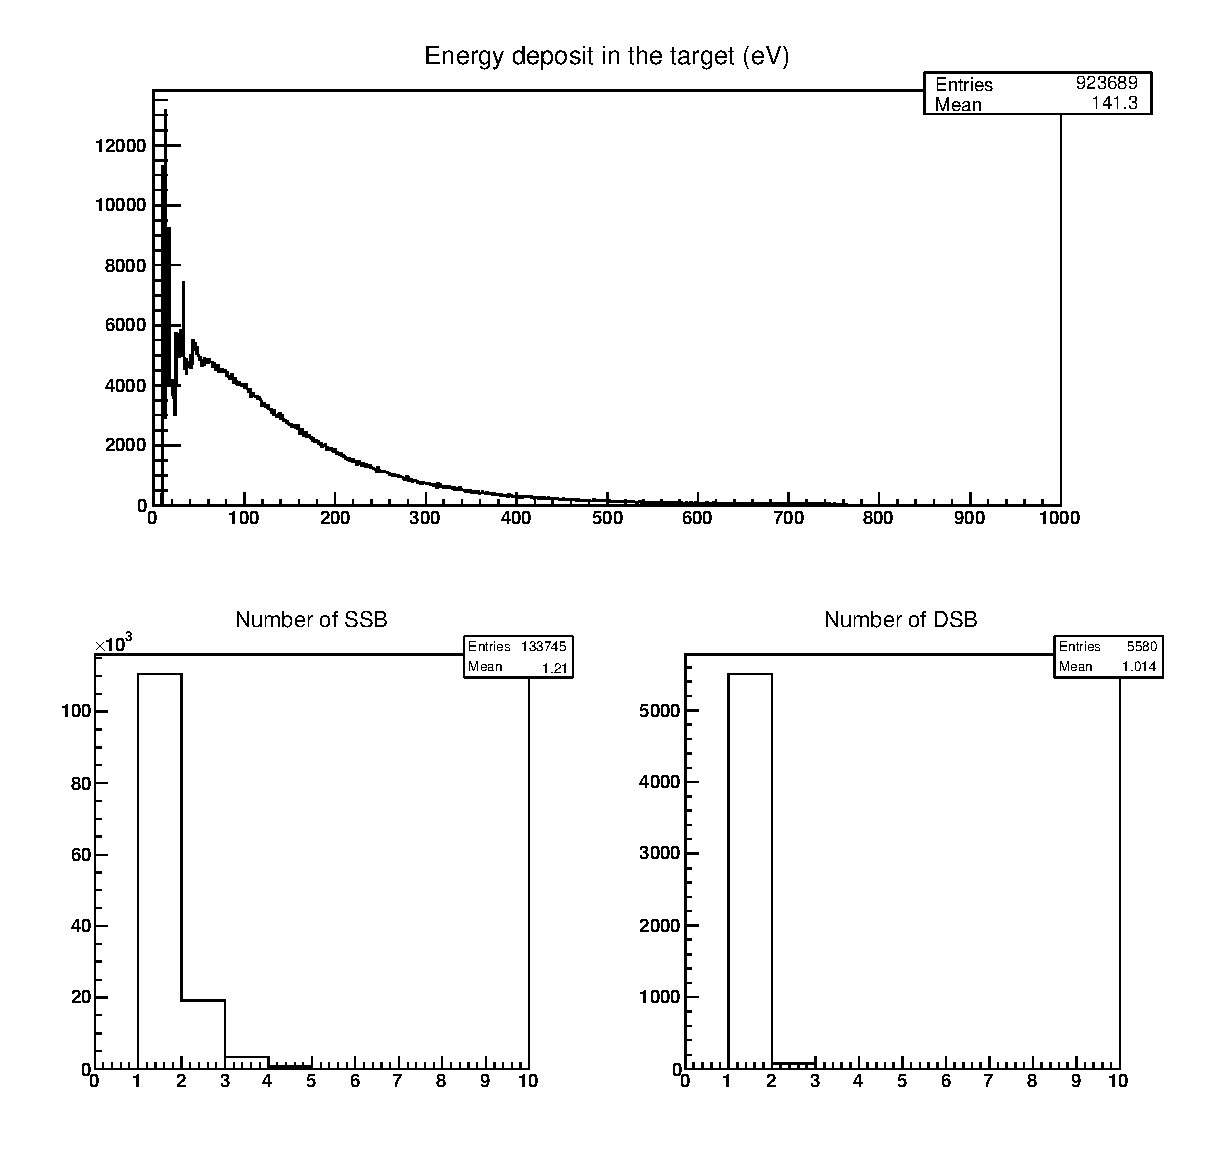
\includegraphics[width=.78\linewidth]{./Figures/1zbbe800ev.eps}
  \caption{1 keV}
  \label{fig:subei6}
\end{subfigure}
\begin{subfigure}{.5\textwidth}
  \centering
  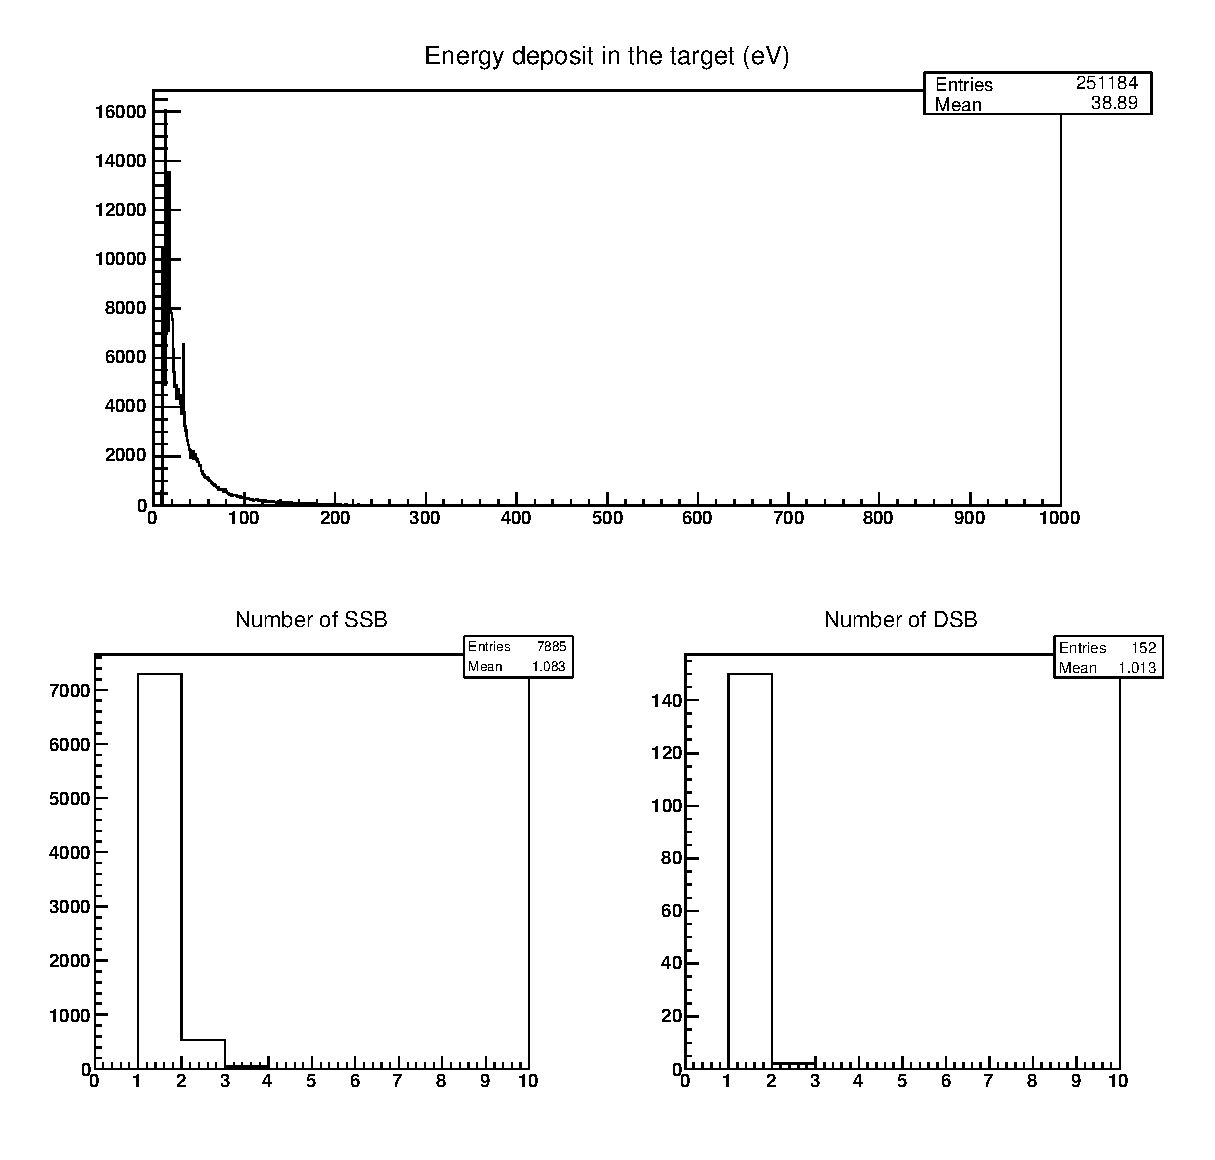
\includegraphics[width=.78\linewidth]{./Figures/1zbbe20kev.eps}
  \caption{20 keV}
  \label{fig:subei7}
\end{subfigure}%
\begin{subfigure}{.5\textwidth}
  \centering
  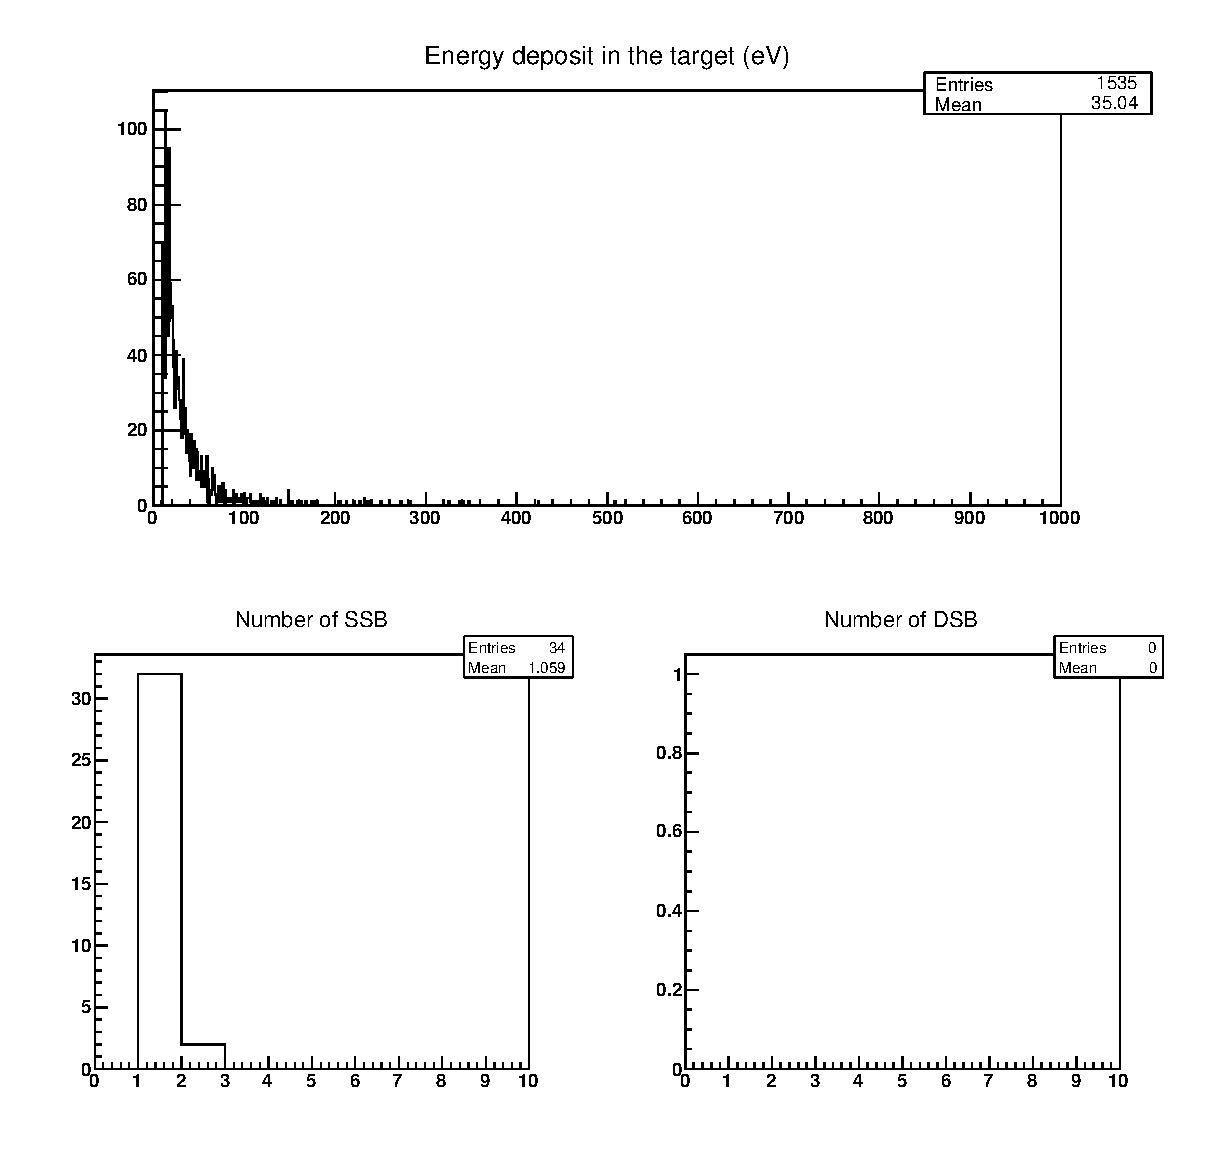
\includegraphics[width=.78\linewidth]{./Figures/1zbbe40kev.eps}
  \caption{40 keV}
  \label{fig:subei8}
\end{subfigure}
\caption{Rompimientos simples y dobles para 1ZBB ($e-$)}
\label{fig:e}
\end{figure}




\begin{figure}
\centering
\begin{subfigure}{.5\textwidth}
  \centering
  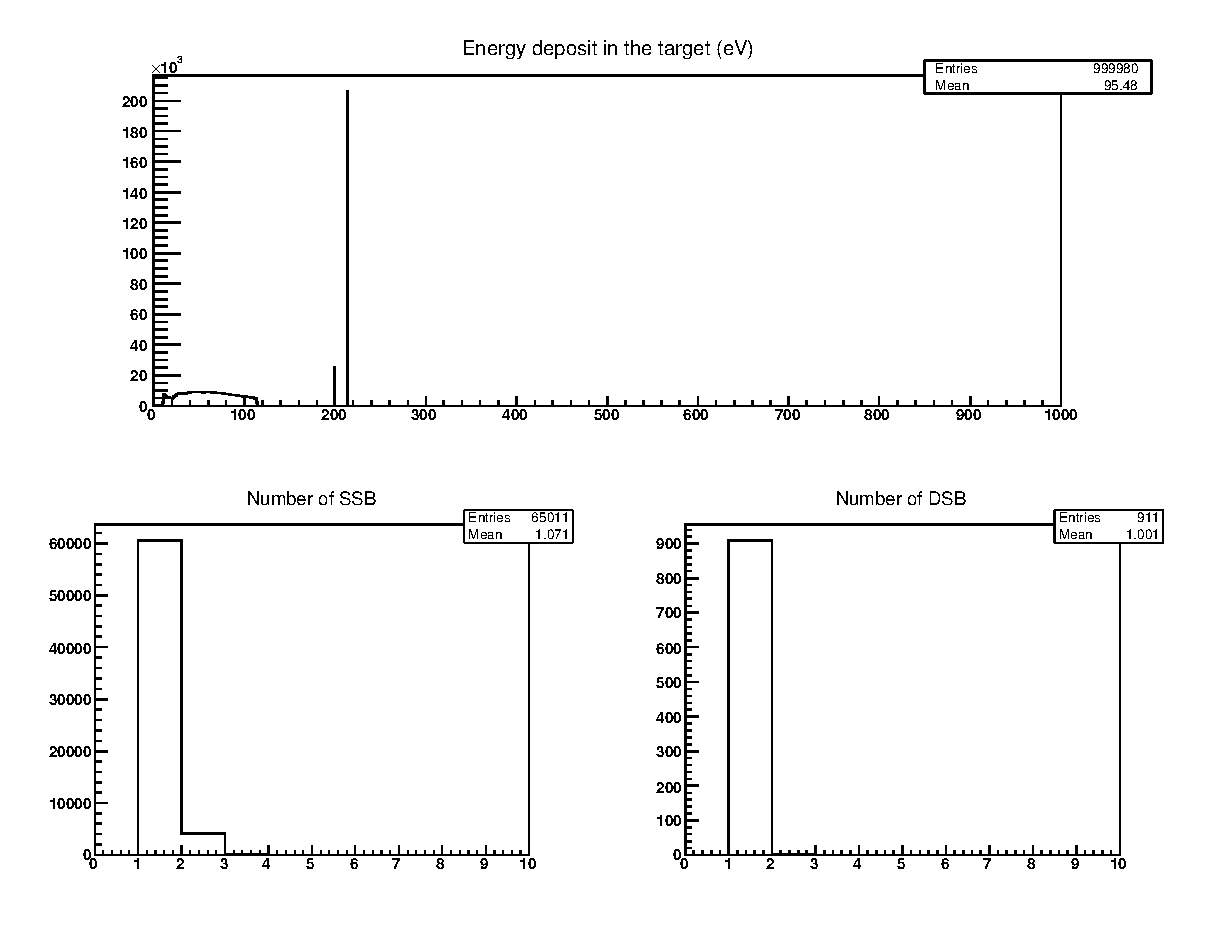
\includegraphics[width=.78\linewidth]{./Figures/1zbbp200ev.eps}
  \caption{200 eV}
  \label{fig:sub1}
\end{subfigure}%
\begin{subfigure}{.5\textwidth}
  \centering
  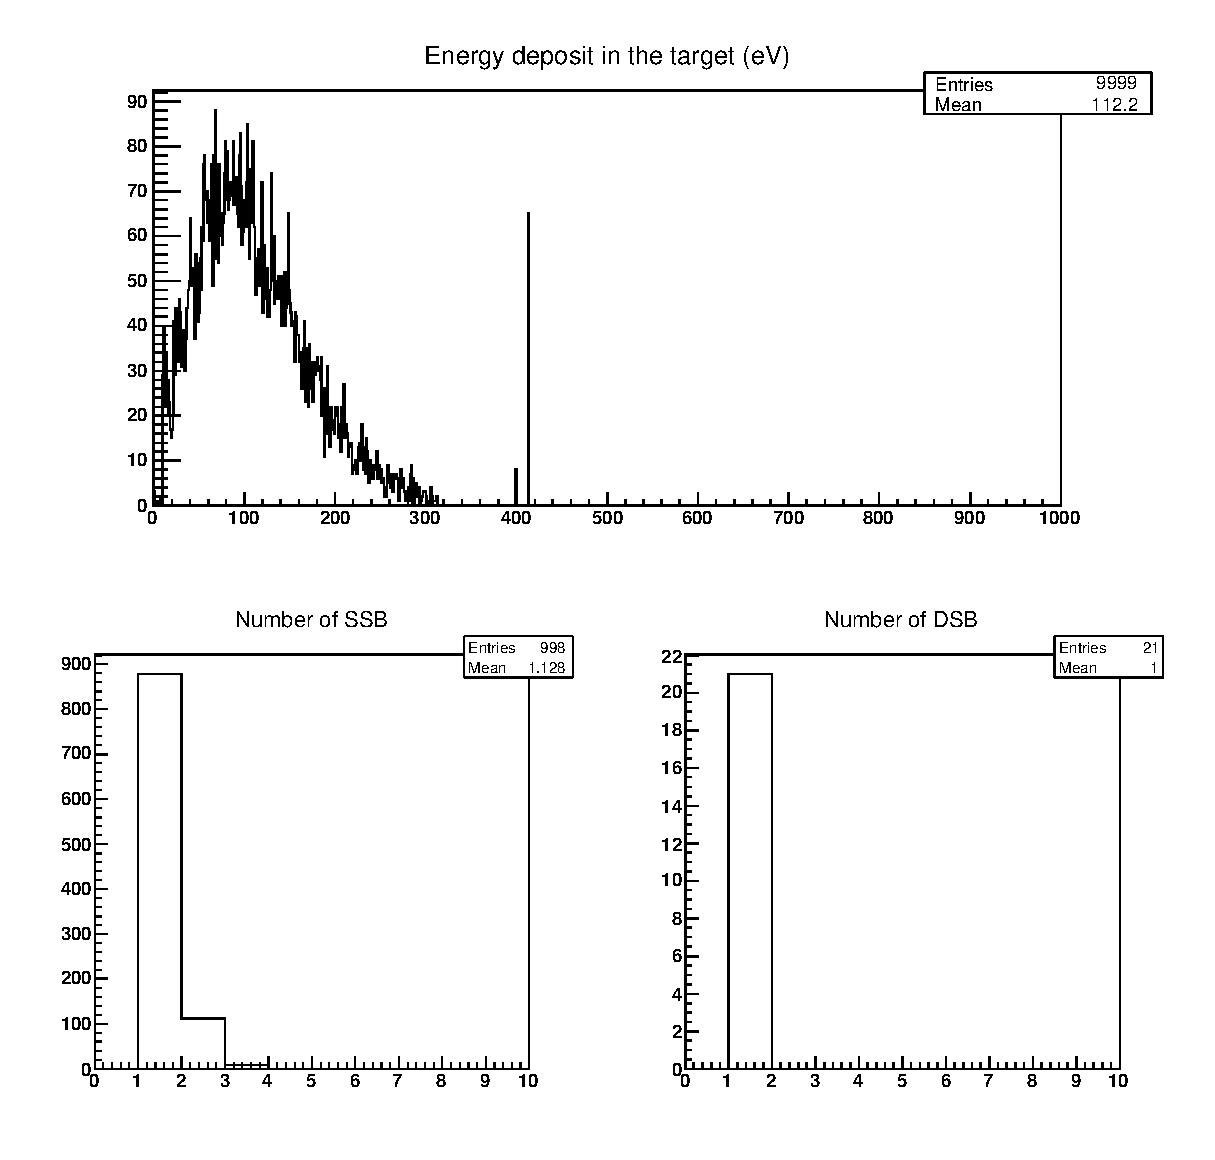
\includegraphics[width=.78\linewidth]{./Figures/1zbbp400ev.eps}
  \caption{400 eV}
  \label{fig:sub2}
\end{subfigure}
\begin{subfigure}{.5\textwidth}
  \centering
  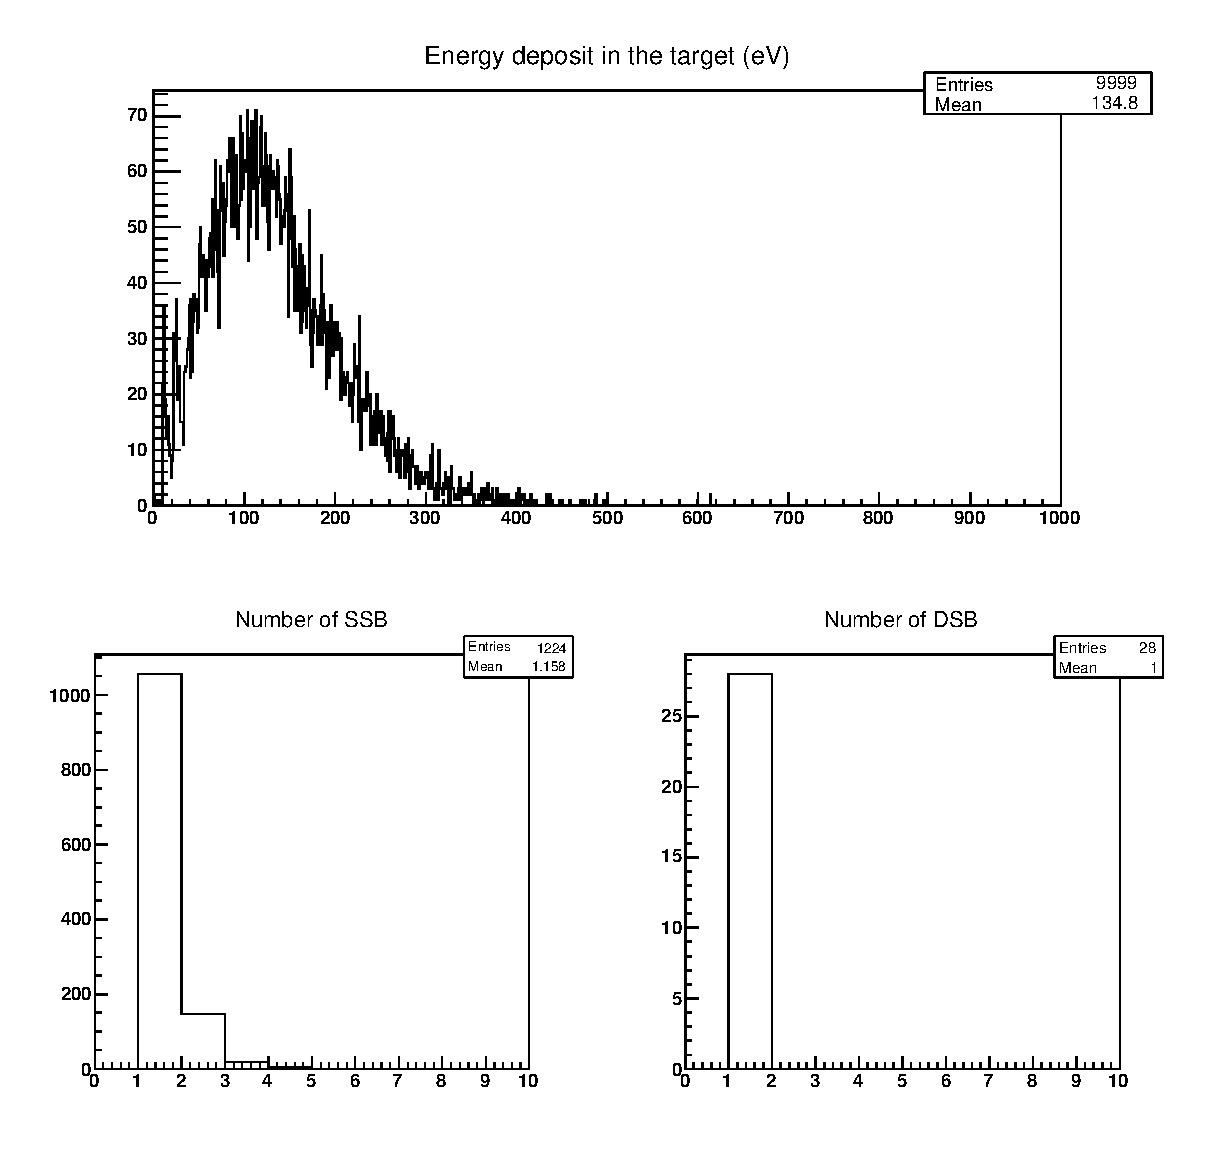
\includegraphics[width=.78\linewidth]{./Figures/1zbbp600ev.eps}
  \caption{600 eV}
  \label{fig:sub3}
\end{subfigure}%
\begin{subfigure}{.5\textwidth}
  \centering
  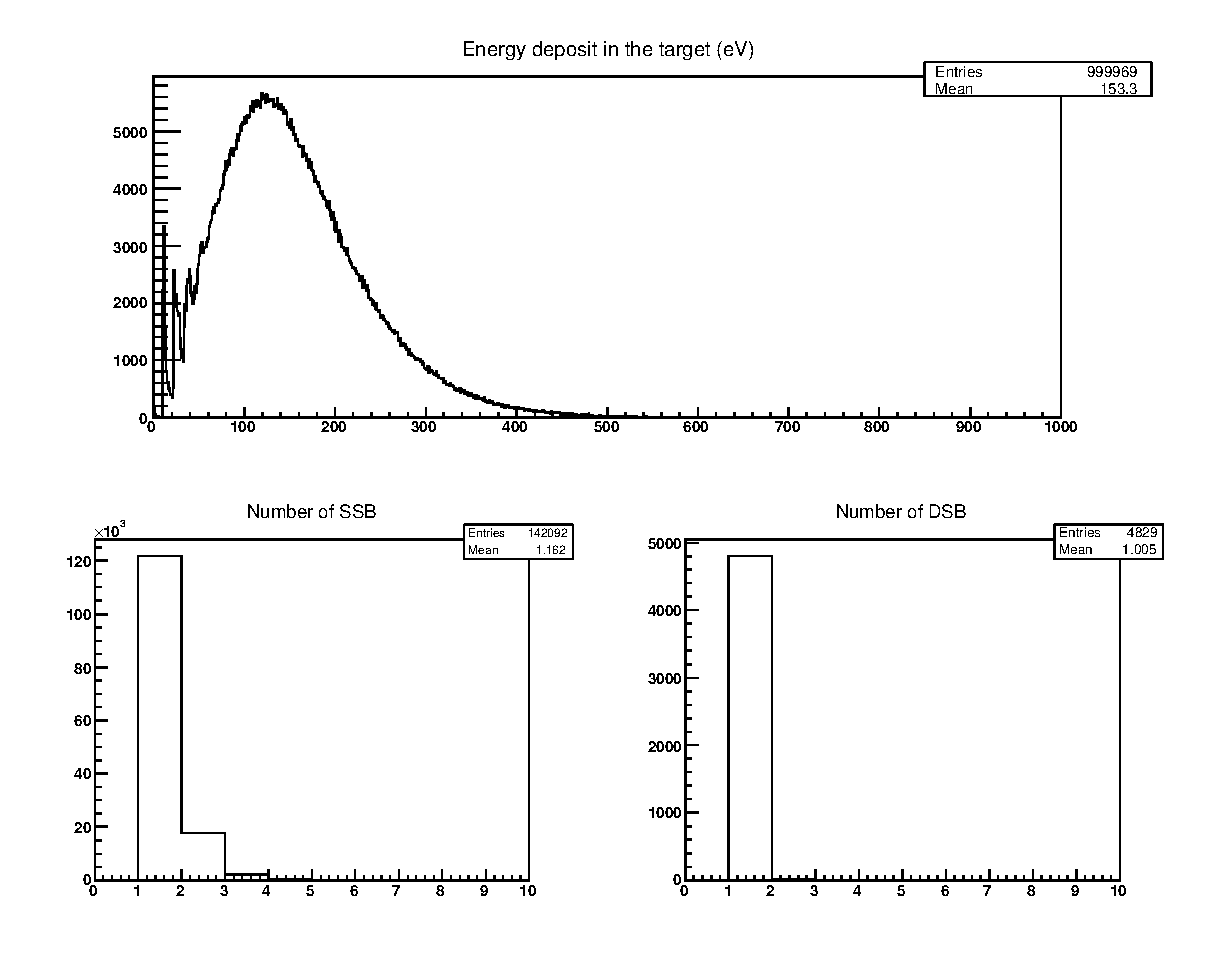
\includegraphics[width=.78\linewidth]{./Figures/1zbbp800ev.eps}
  \caption{800 eV}
  \label{fig:sub4}
\end{subfigure}
\begin{subfigure}{.5\textwidth}
  \centering
  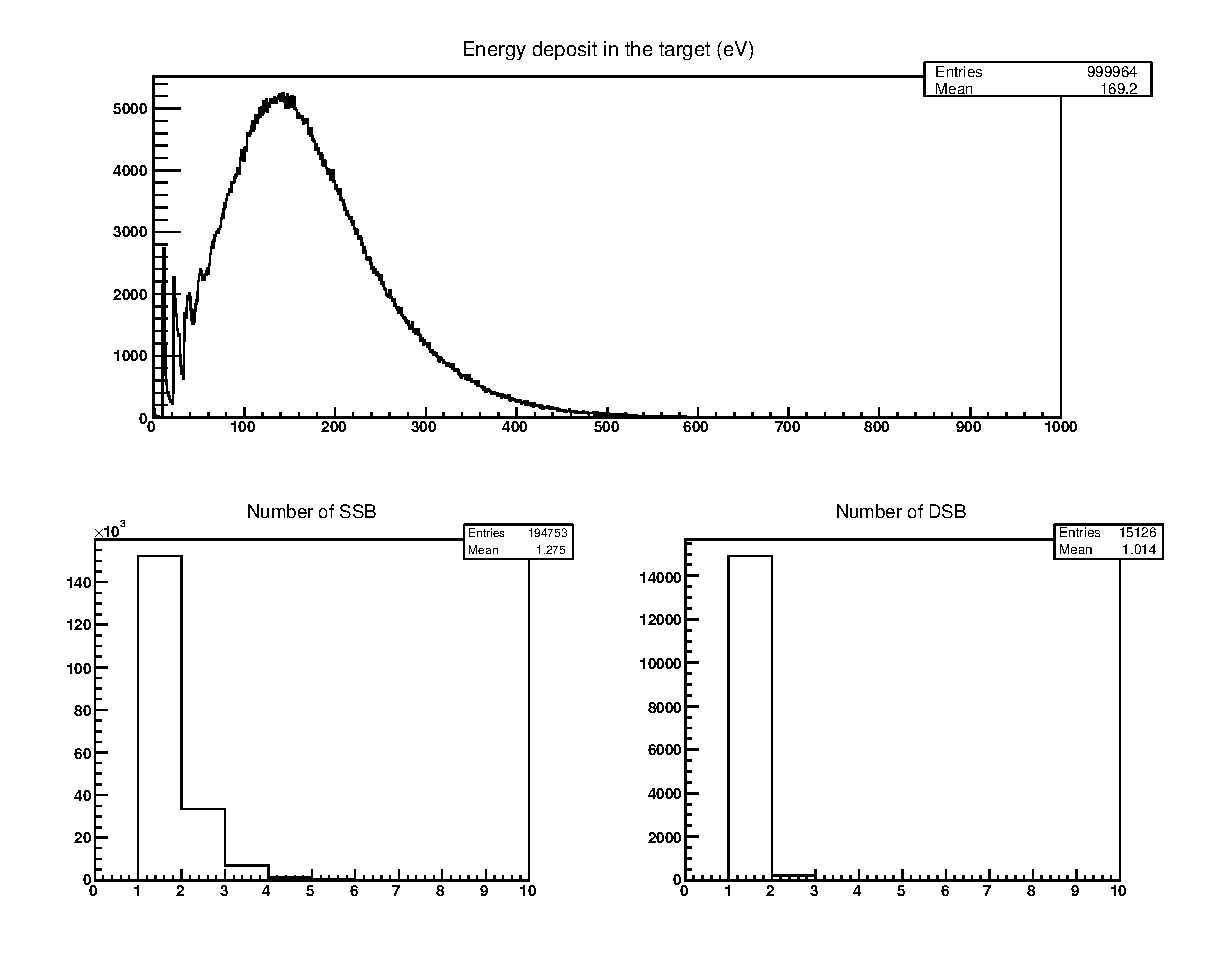
\includegraphics[width=.78\linewidth]{./Figures/1zbbp1kev.eps}
  \caption{1 keV}
  \label{fig:sub5}
\end{subfigure}%
\begin{subfigure}{.5\textwidth}
  \centering
  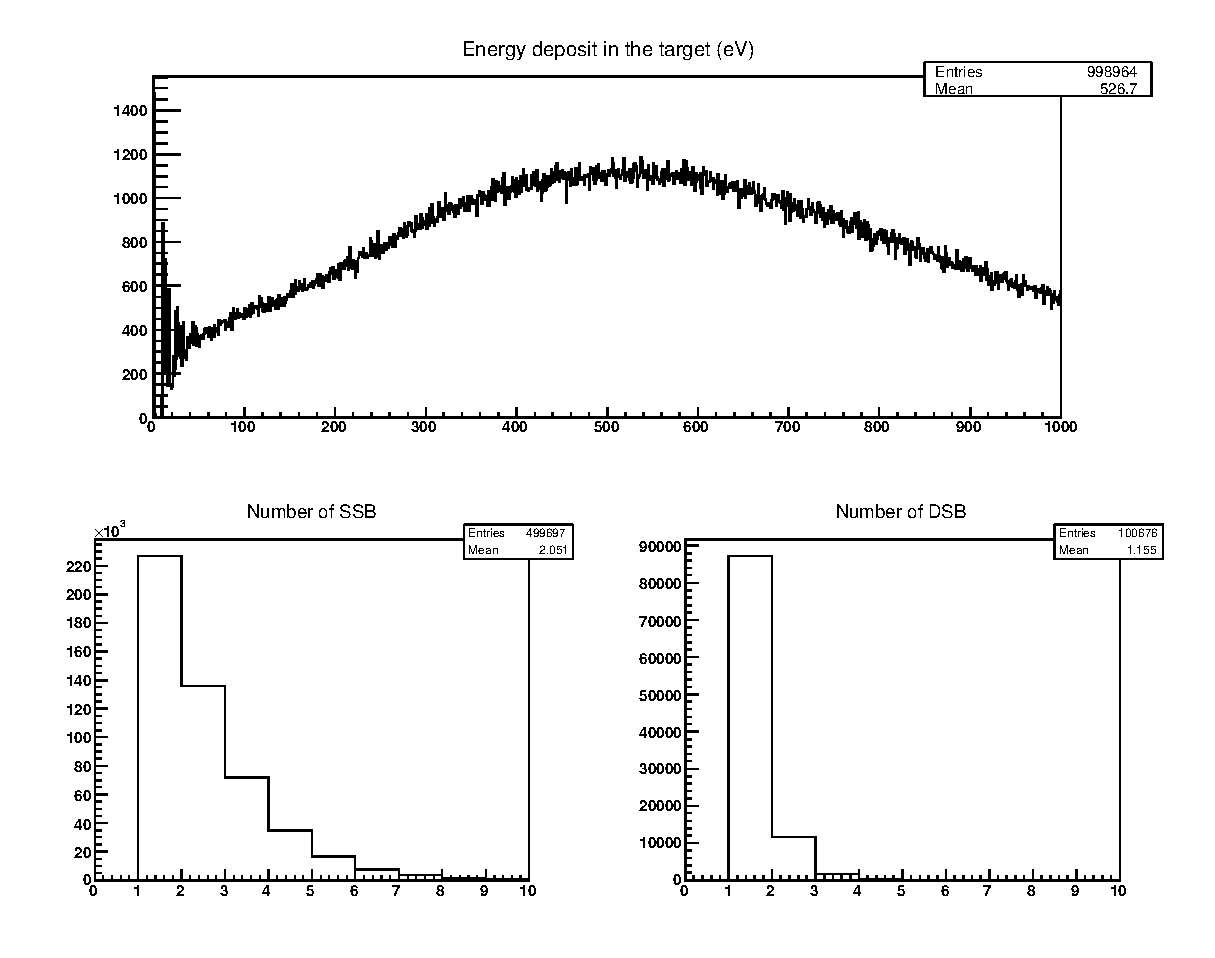
\includegraphics[width=.78\linewidth]{./Figures/1zbbp200kev.eps}
  \caption{200 keV}
  \label{fig:sub6}
\end{subfigure}
\begin{subfigure}{.5\textwidth}
  \centering
  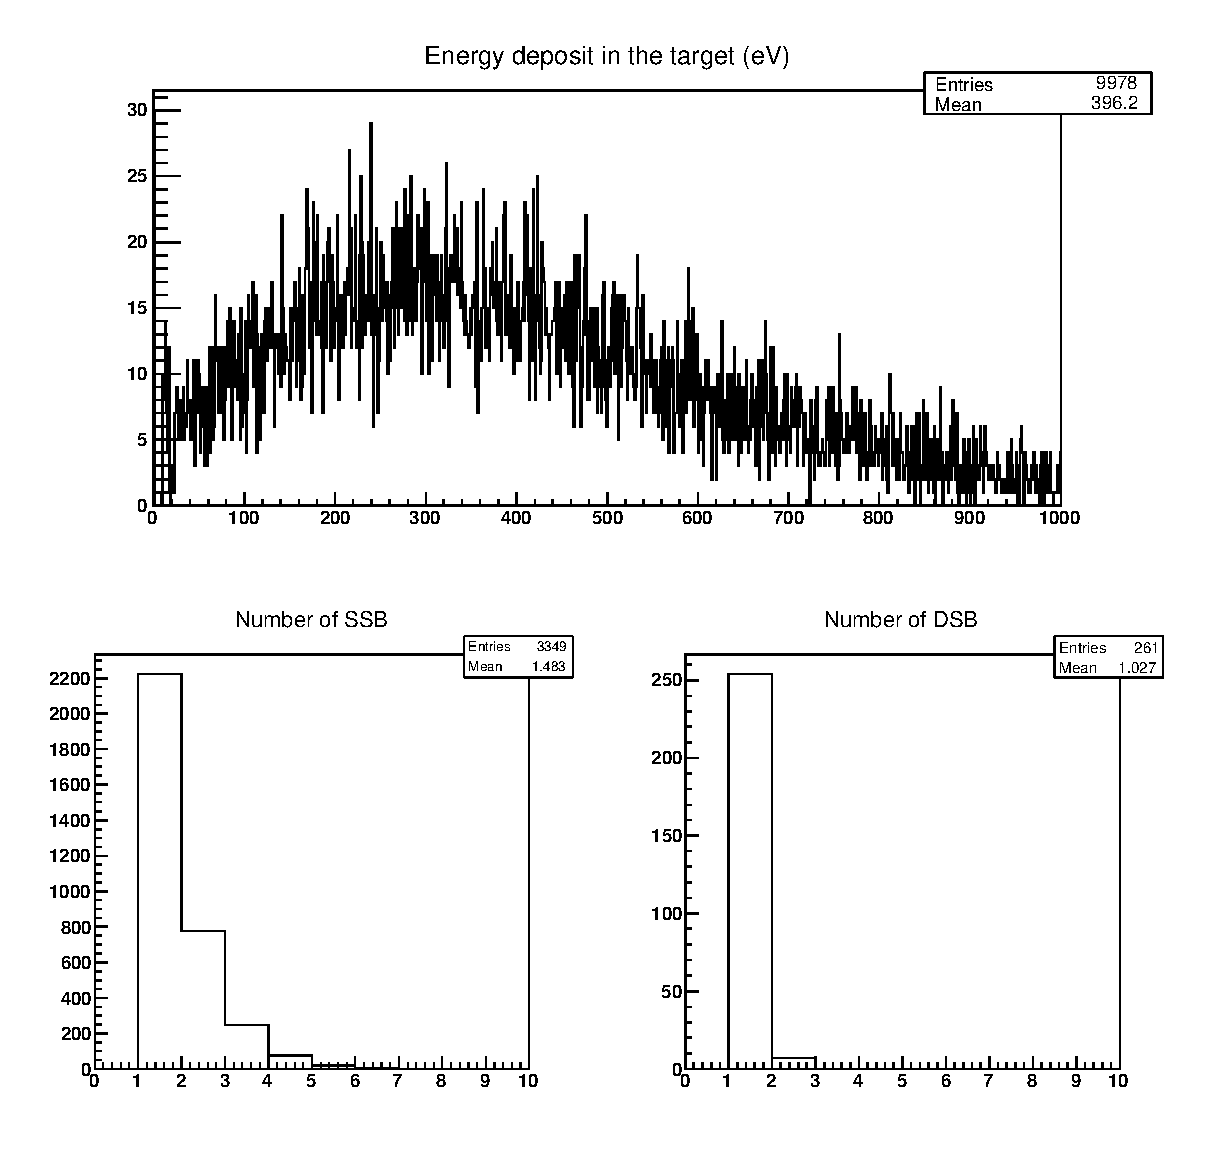
\includegraphics[width=.78\linewidth]{./Figures/1zbbp400kev.eps}
  \caption{400 keV}
  \label{fig:sub7}
\end{subfigure}%
\begin{subfigure}{.5\textwidth}
  \centering
  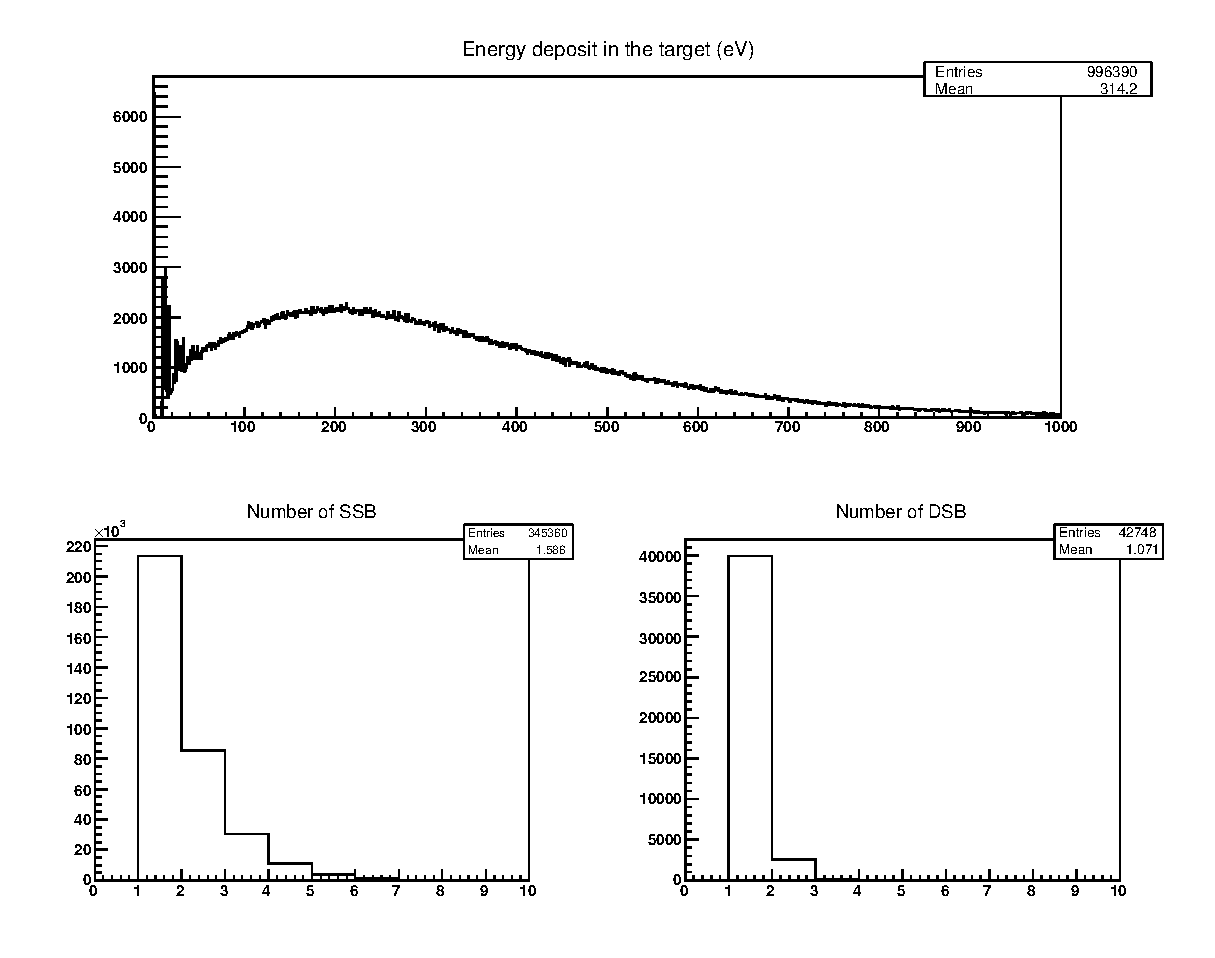
\includegraphics[width=.78\linewidth]{./Figures/1zbbp600kev.eps}
  \caption{600 keV}
  \label{fig:sub8}
\end{subfigure}
\caption{Rompimientos simples y dobles para 1ZBB ($proton$)}
\label{fig:p}
\end{figure}



\begin{figure}
\centering
\begin{subfigure}{.5\textwidth}
  \centering
  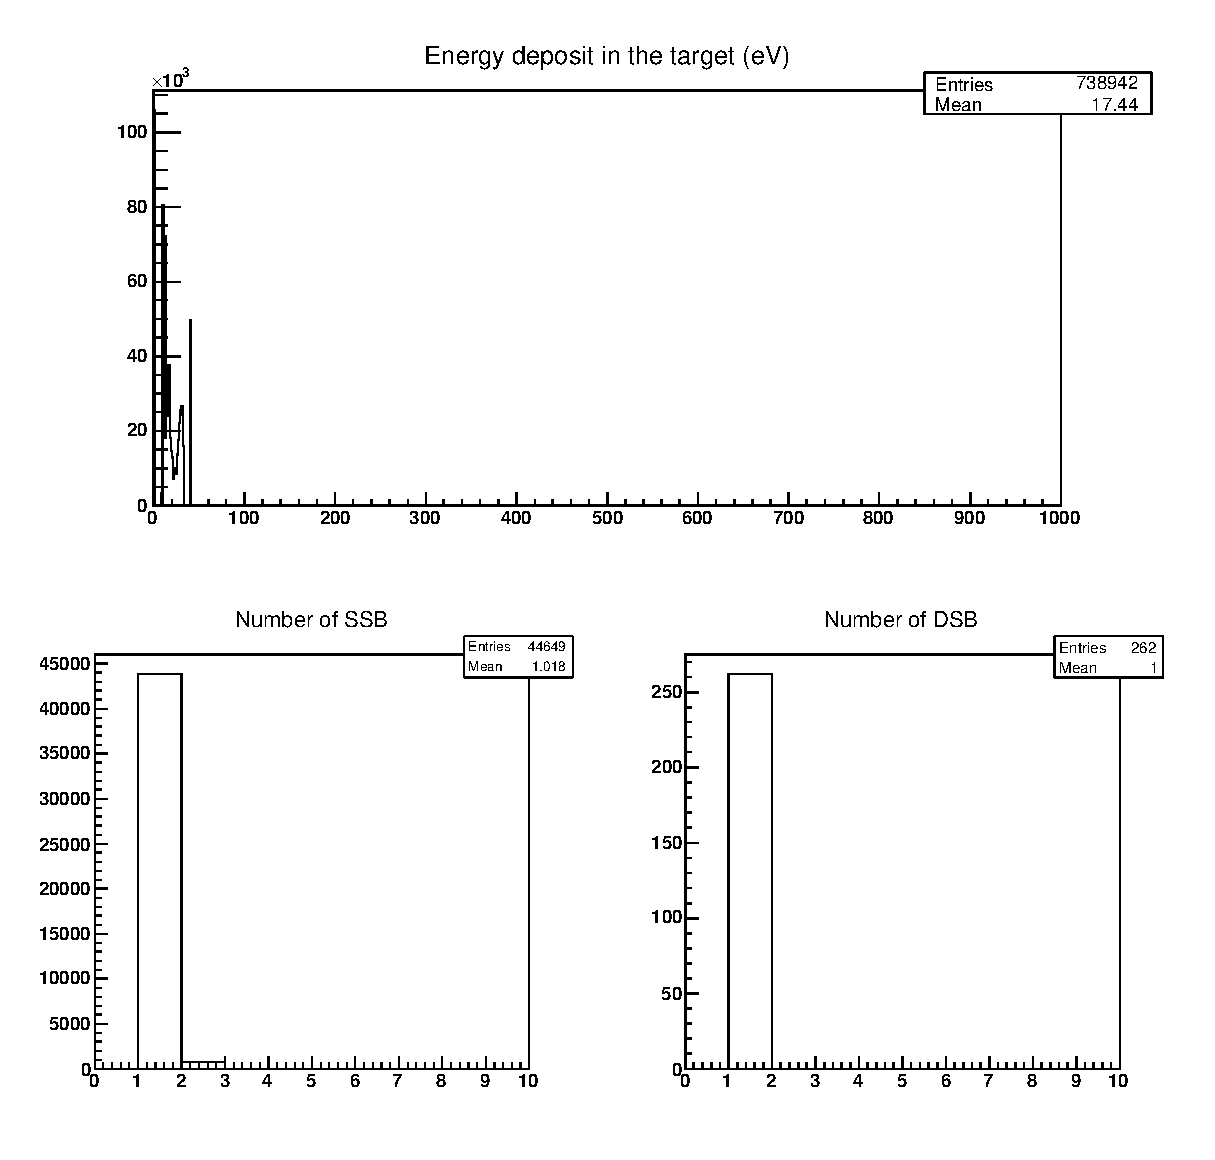
\includegraphics[width=.78\linewidth]{./Figures/1fzxe40ev.eps}
  \caption{40 eV}
  \label{fig:sube1}
\end{subfigure}%
\begin{subfigure}{.5\textwidth}
  \centering
  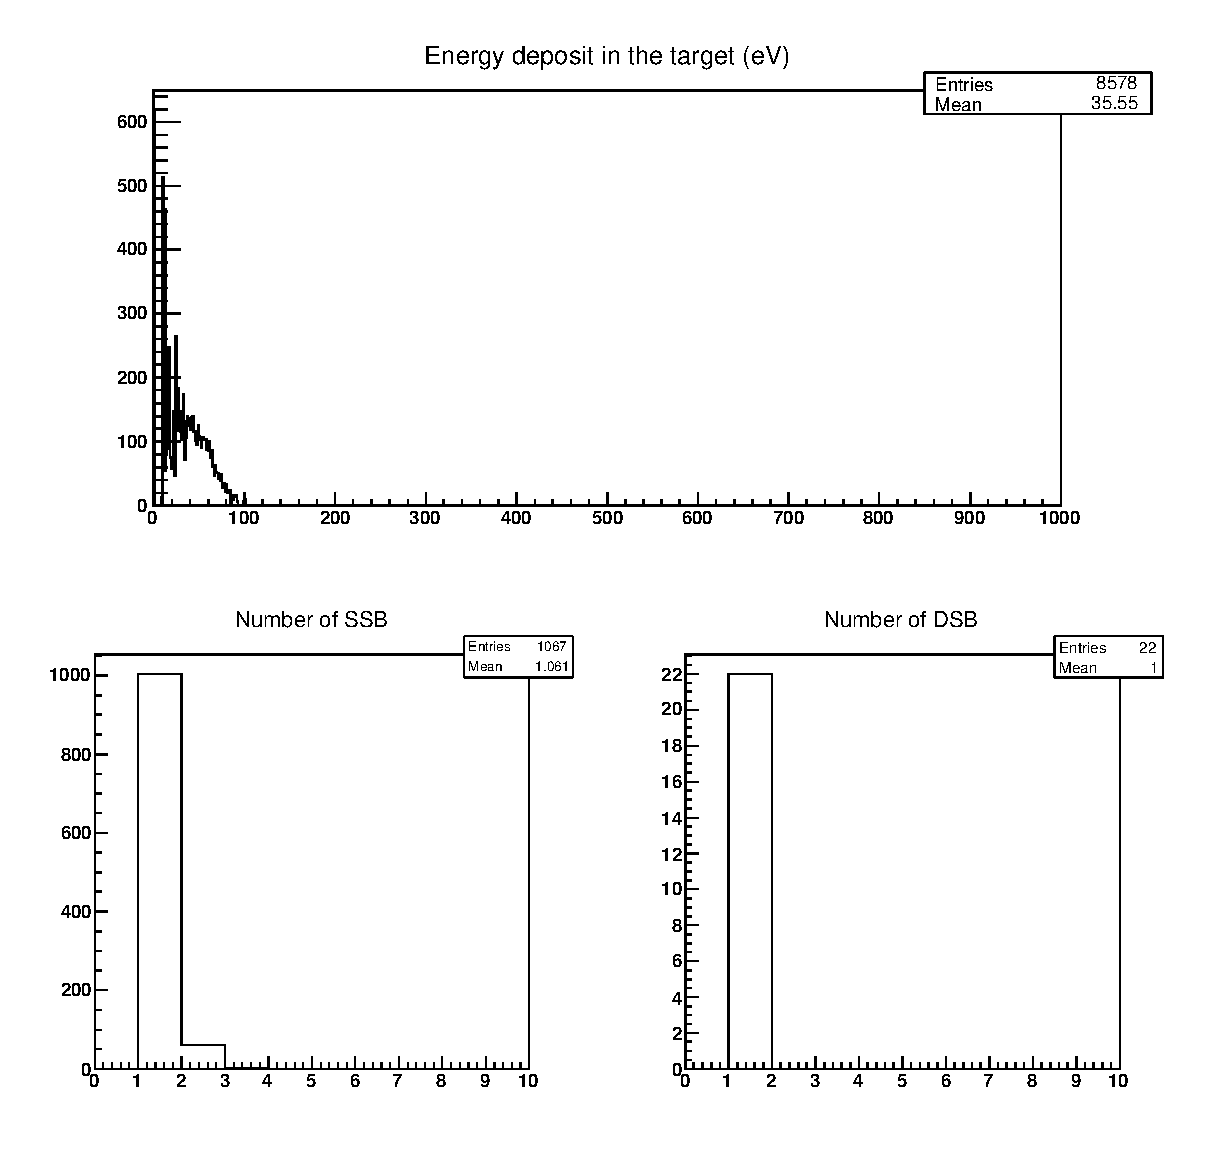
\includegraphics[width=.78\linewidth]{./Figures/1fzxe100ev.eps}
  \caption{100 eV}
  \label{fig:sube2}
\end{subfigure}
\begin{subfigure}{.5\textwidth}
  \centering
  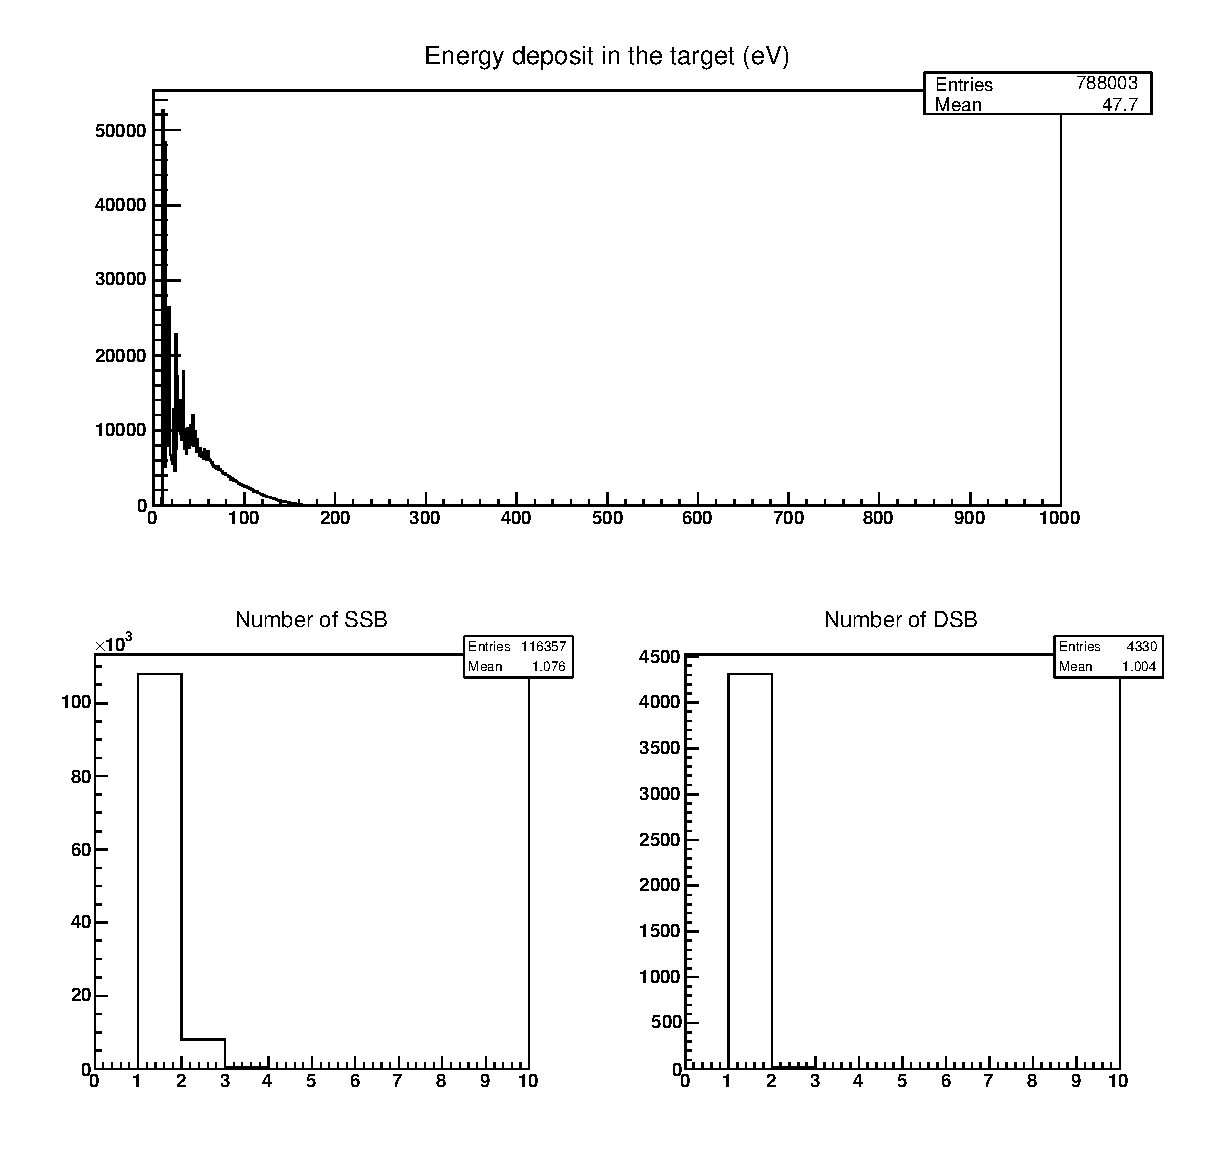
\includegraphics[width=.78\linewidth]{./Figures/1fzxe200ev.eps}
  \caption{200 eV}
  \label{fig:sube3}
\end{subfigure}%
\begin{subfigure}{.5\textwidth}
  \centering
  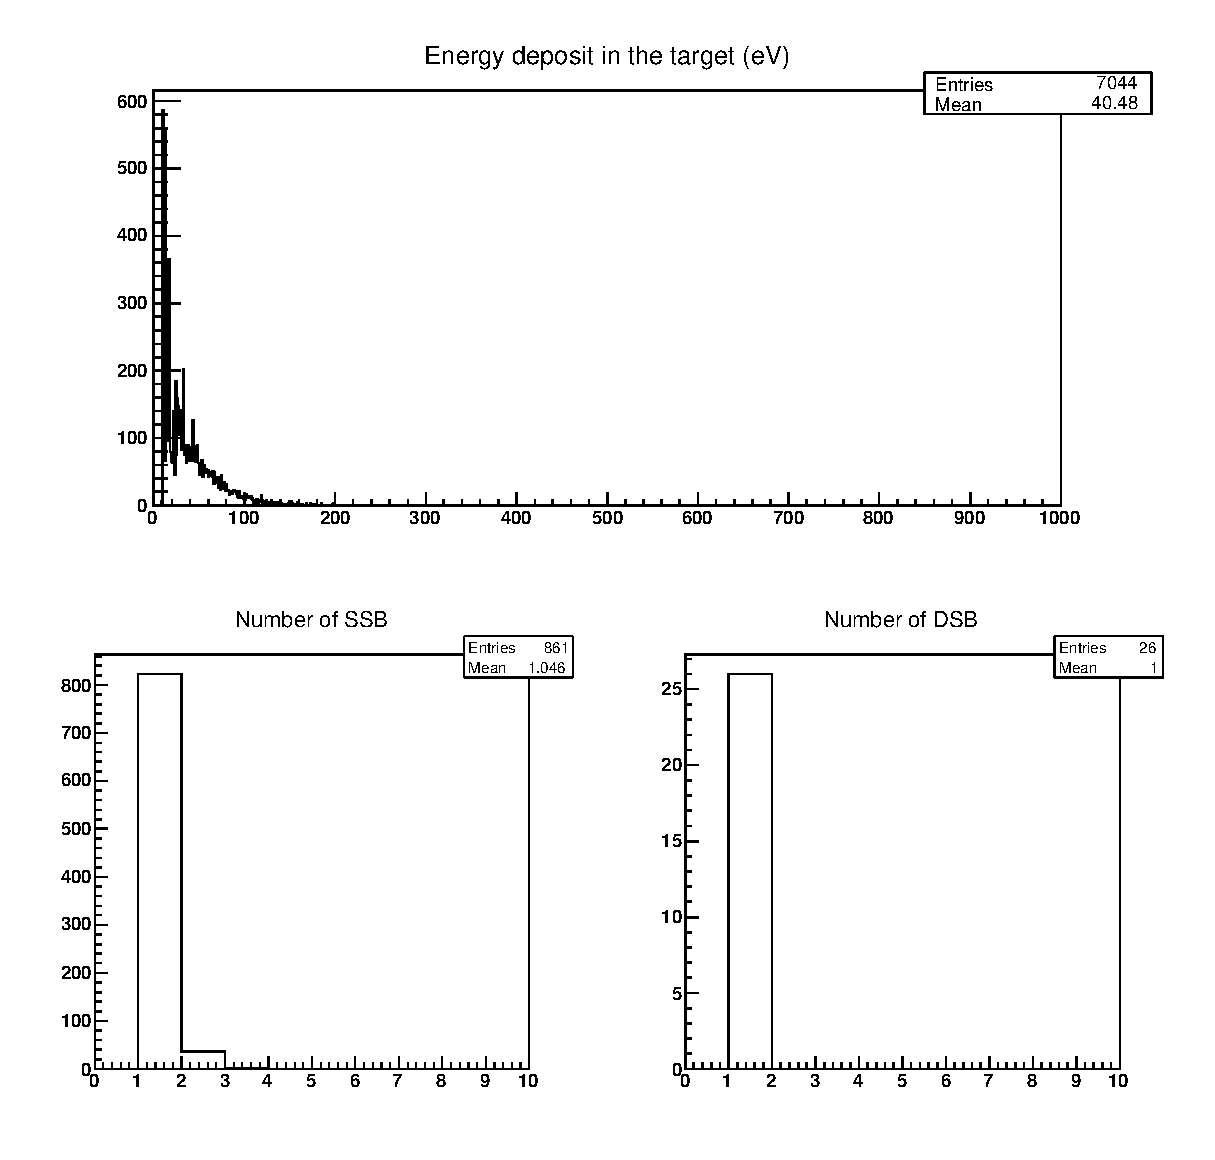
\includegraphics[width=.78\linewidth]{./Figures/1fzxe400ev.eps}
  \caption{400 eV}
  \label{fig:sube4}
\end{subfigure}
\begin{subfigure}{.5\textwidth}
  \centering
  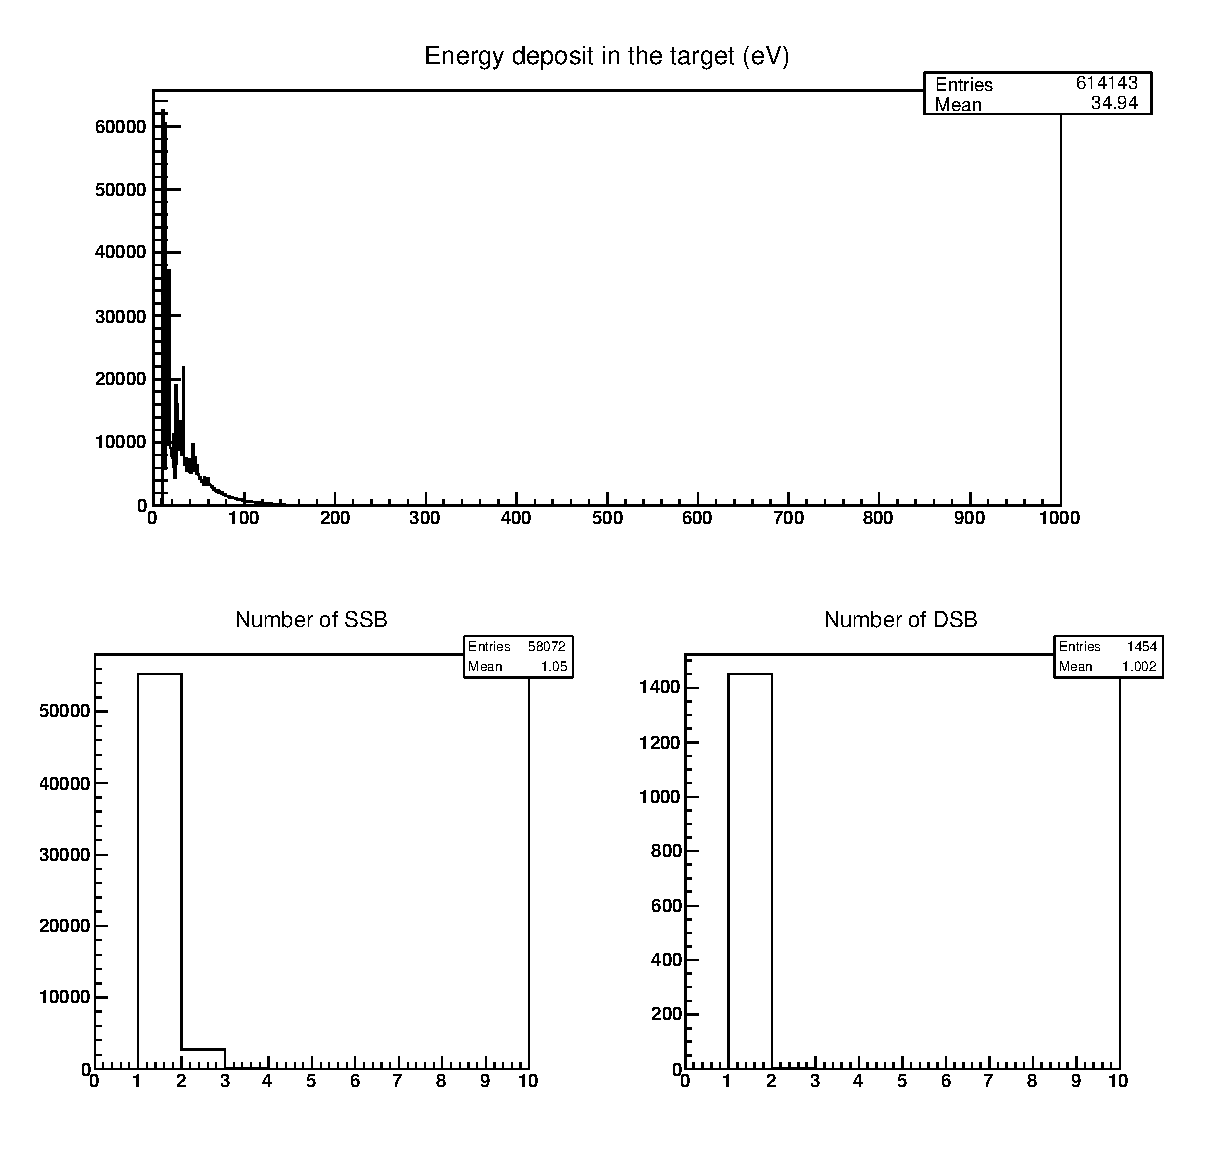
\includegraphics[width=.78\linewidth]{./Figures/1fzxe600ev.eps}
  \caption{600 eV}
  \label{fig:sube5}
\end{subfigure}%
\begin{subfigure}{.5\textwidth}
  \centering
  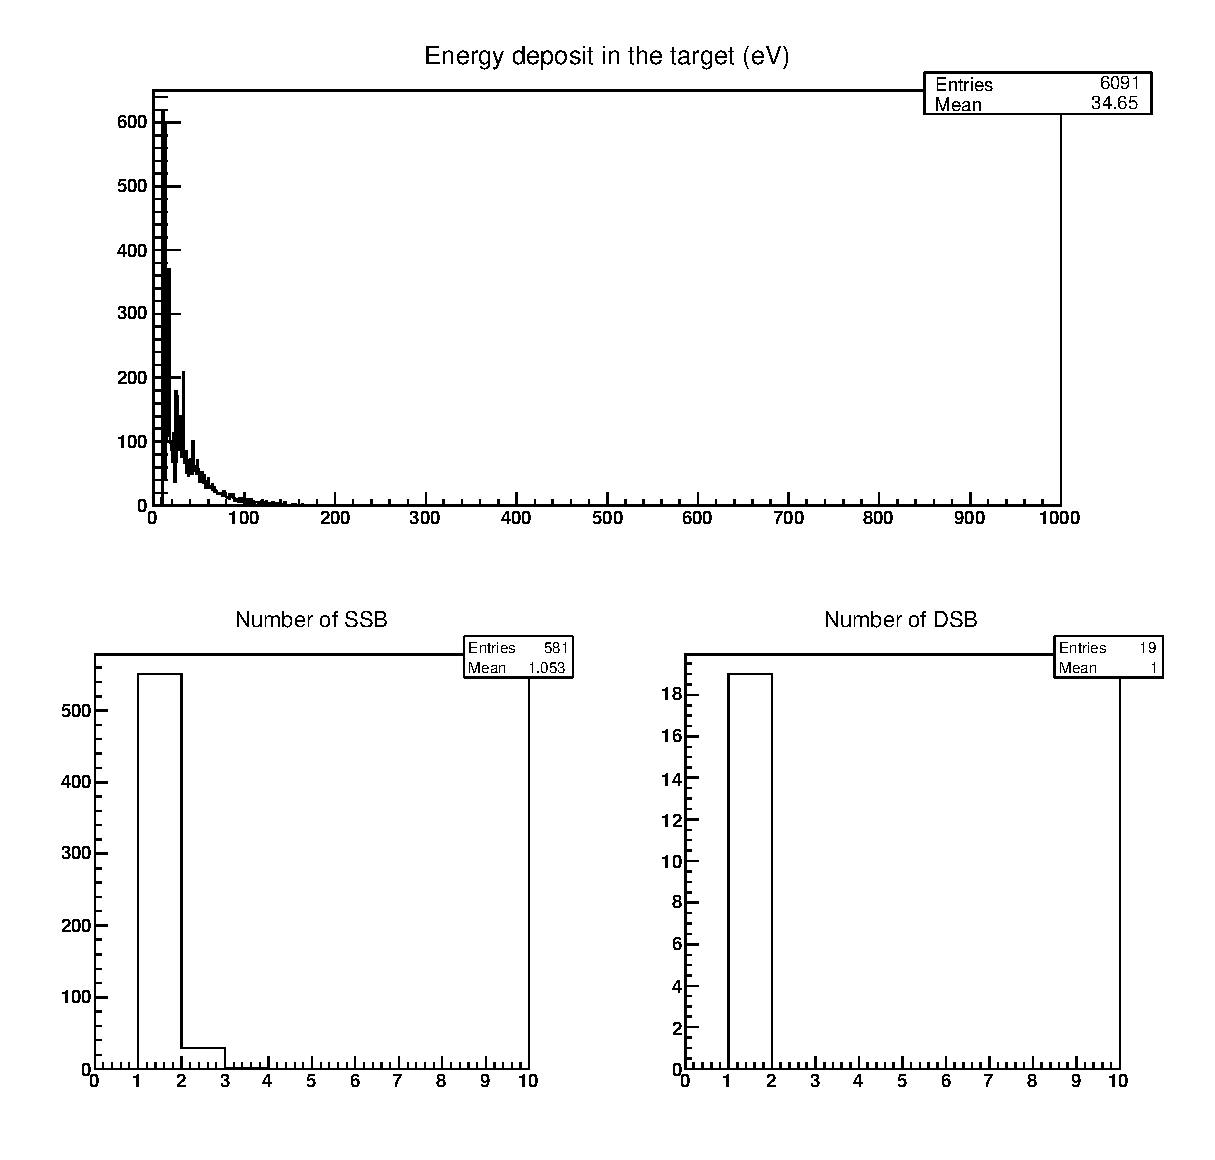
\includegraphics[width=.78\linewidth]{./Figures/1fzxe800ev.eps}
  \caption{800 eV}
  \label{fig:sube6}
\end{subfigure}
\begin{subfigure}{.5\textwidth}
  \centering
  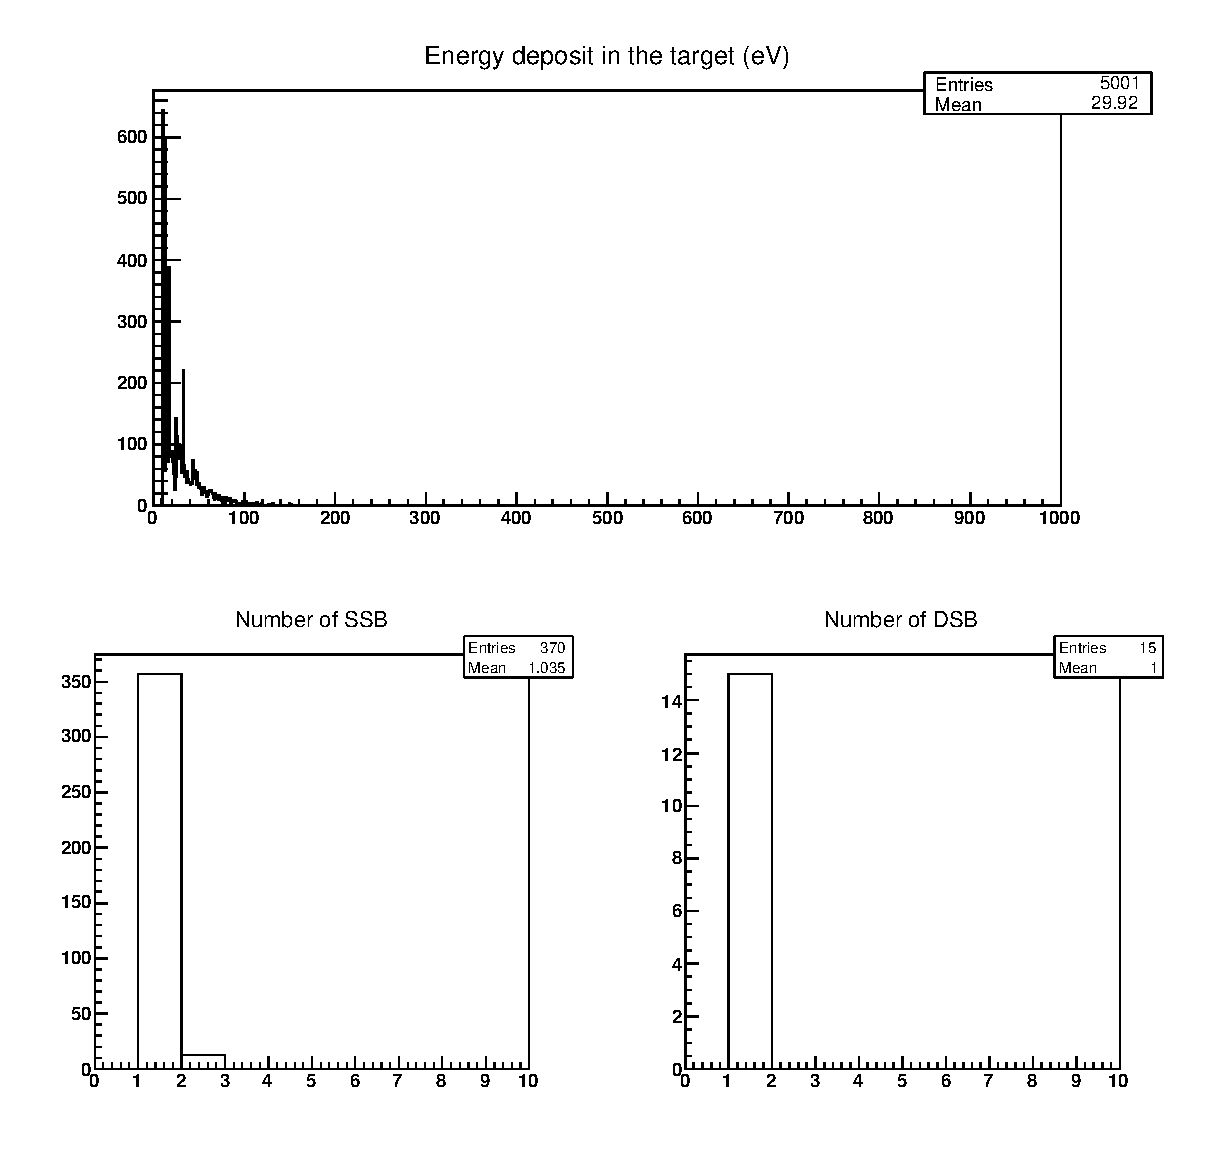
\includegraphics[width=.78\linewidth]{./Figures/1fzxe1kev.eps}
  \caption{1 keV}
  \label{fig:sube7}
\end{subfigure}%
\begin{subfigure}{.5\textwidth}
  \centering
  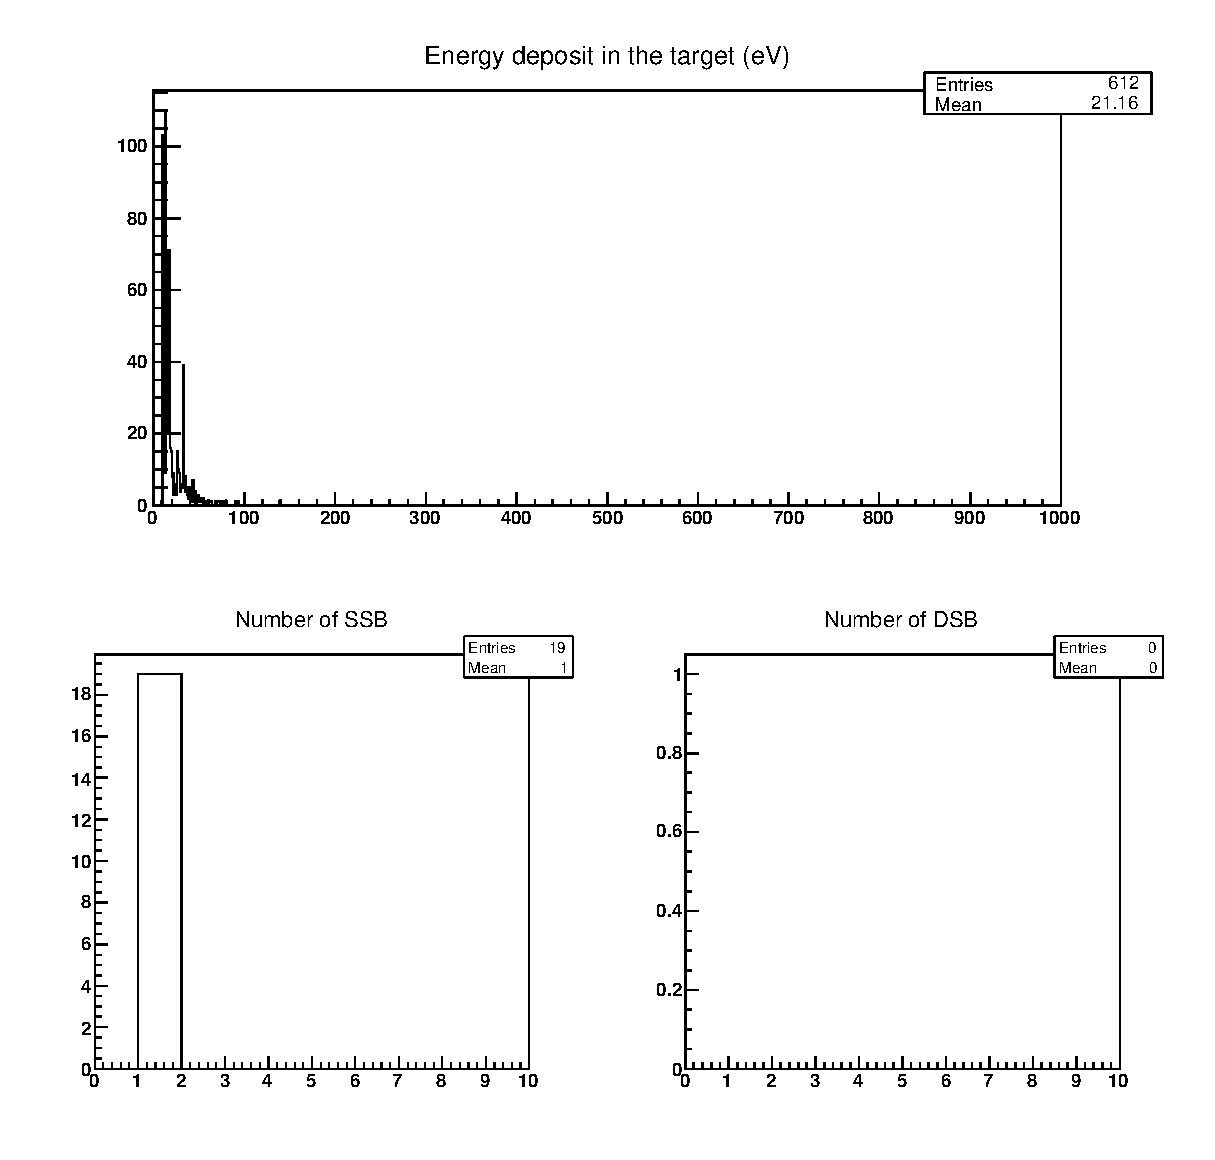
\includegraphics[width=.78\linewidth]{./Figures/1fzxe20kev.eps}
  \caption{20 keV}
  \label{fig:sube8}
\end{subfigure}
\caption{Rompimientos simples y dobles para 1FZX ($e-$)}
\label{fig:e2}
\end{figure}




\begin{figure}
\centering
\begin{subfigure}{.5\textwidth}
  \centering
  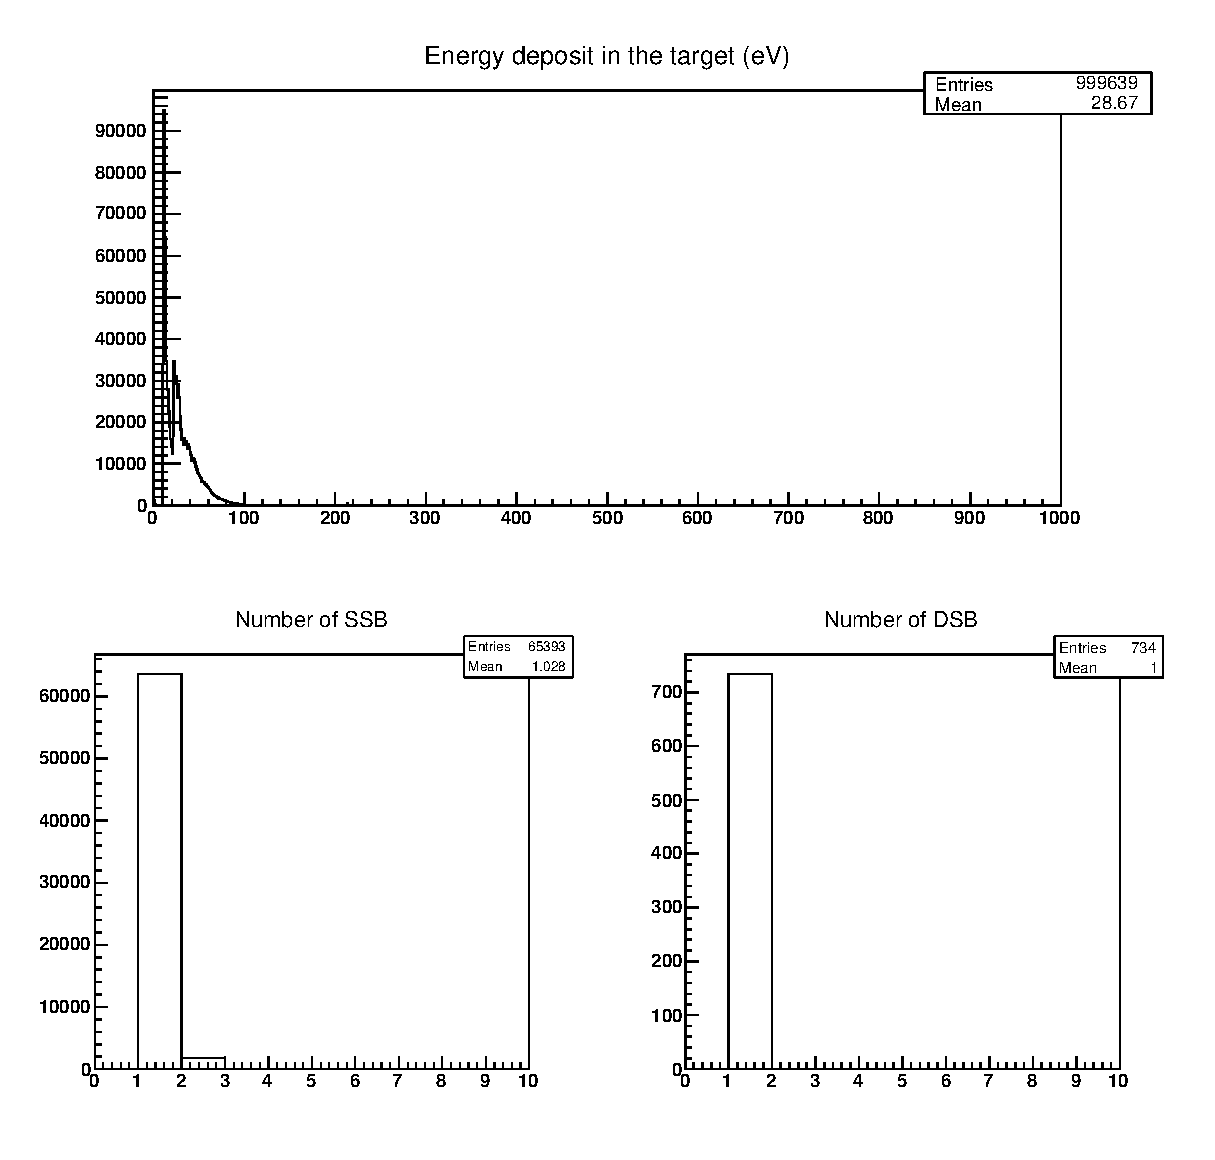
\includegraphics[width=.78\linewidth]{./Figures/1fzxp200ev.eps}
  \caption{200 eV}
  \label{fig:subi1}
\end{subfigure}%
\begin{subfigure}{.5\textwidth}
  \centering
  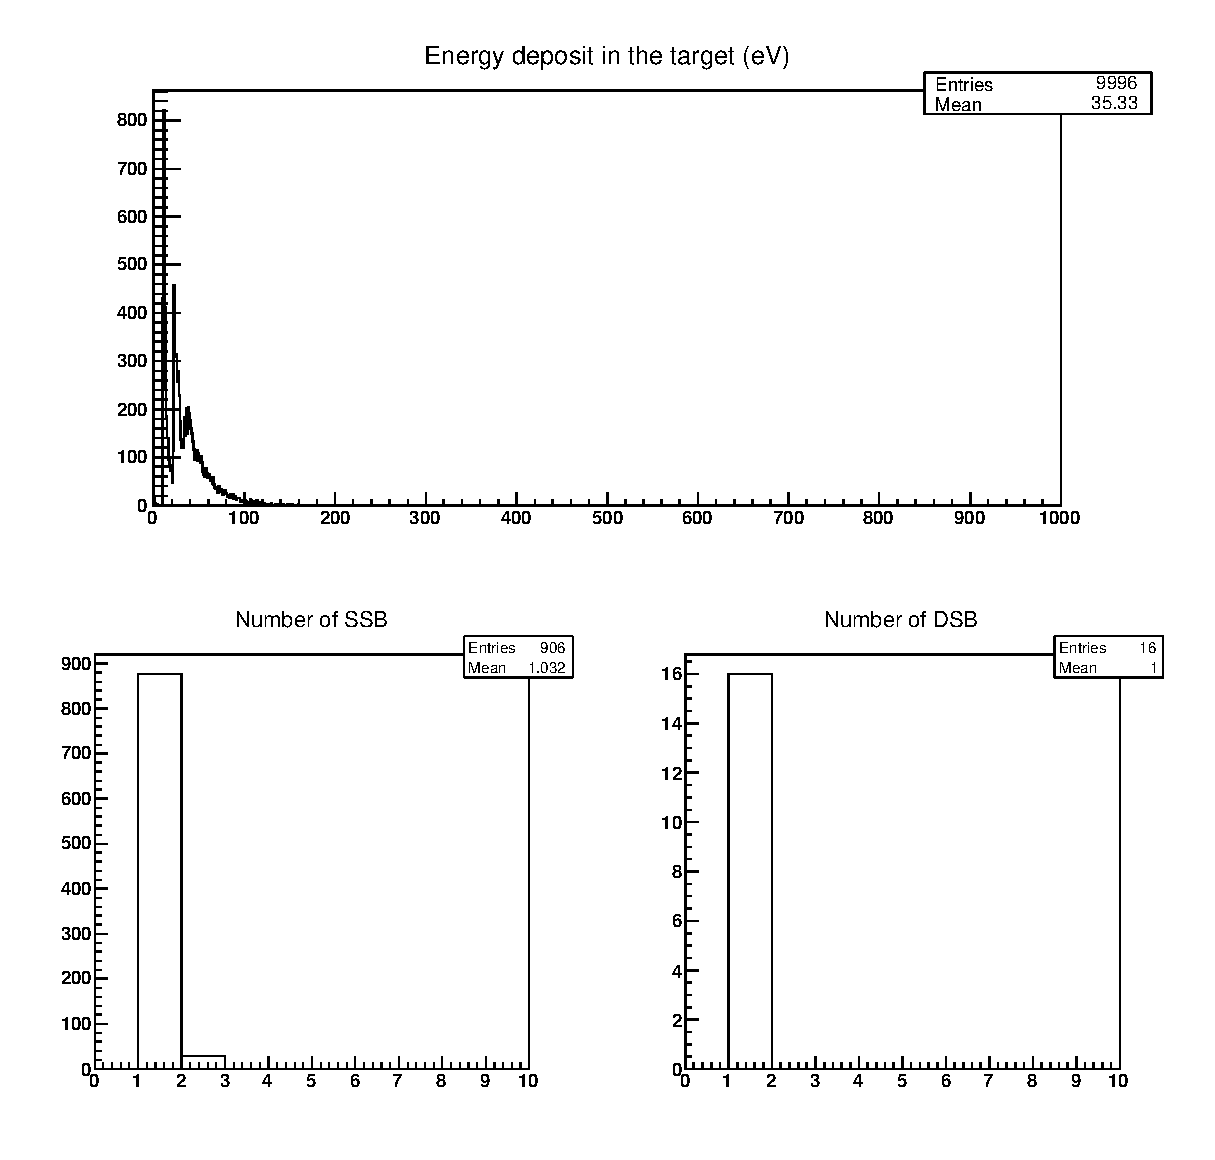
\includegraphics[width=.78\linewidth]{./Figures/1fzxp400ev.eps}
  \caption{400 eV}
  \label{fig:subi2}
\end{subfigure}
\begin{subfigure}{.5\textwidth}
  \centering
  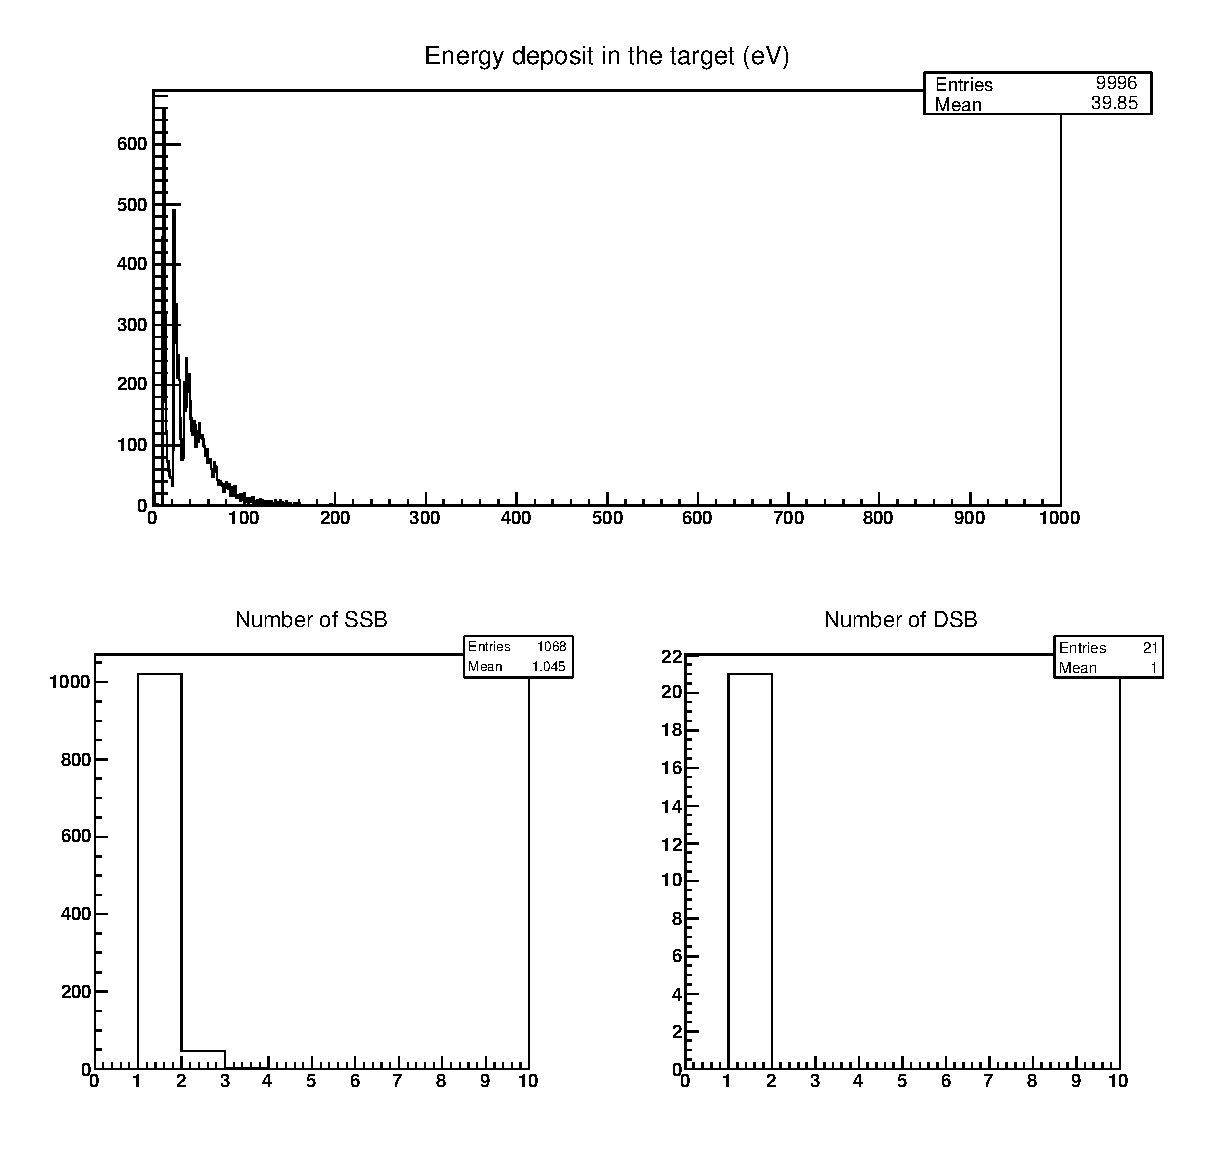
\includegraphics[width=.78\linewidth]{./Figures/1fzxp600ev.eps}
  \caption{600 eV}
  \label{fig:subi3}
\end{subfigure}%
\begin{subfigure}{.5\textwidth}
  \centering
  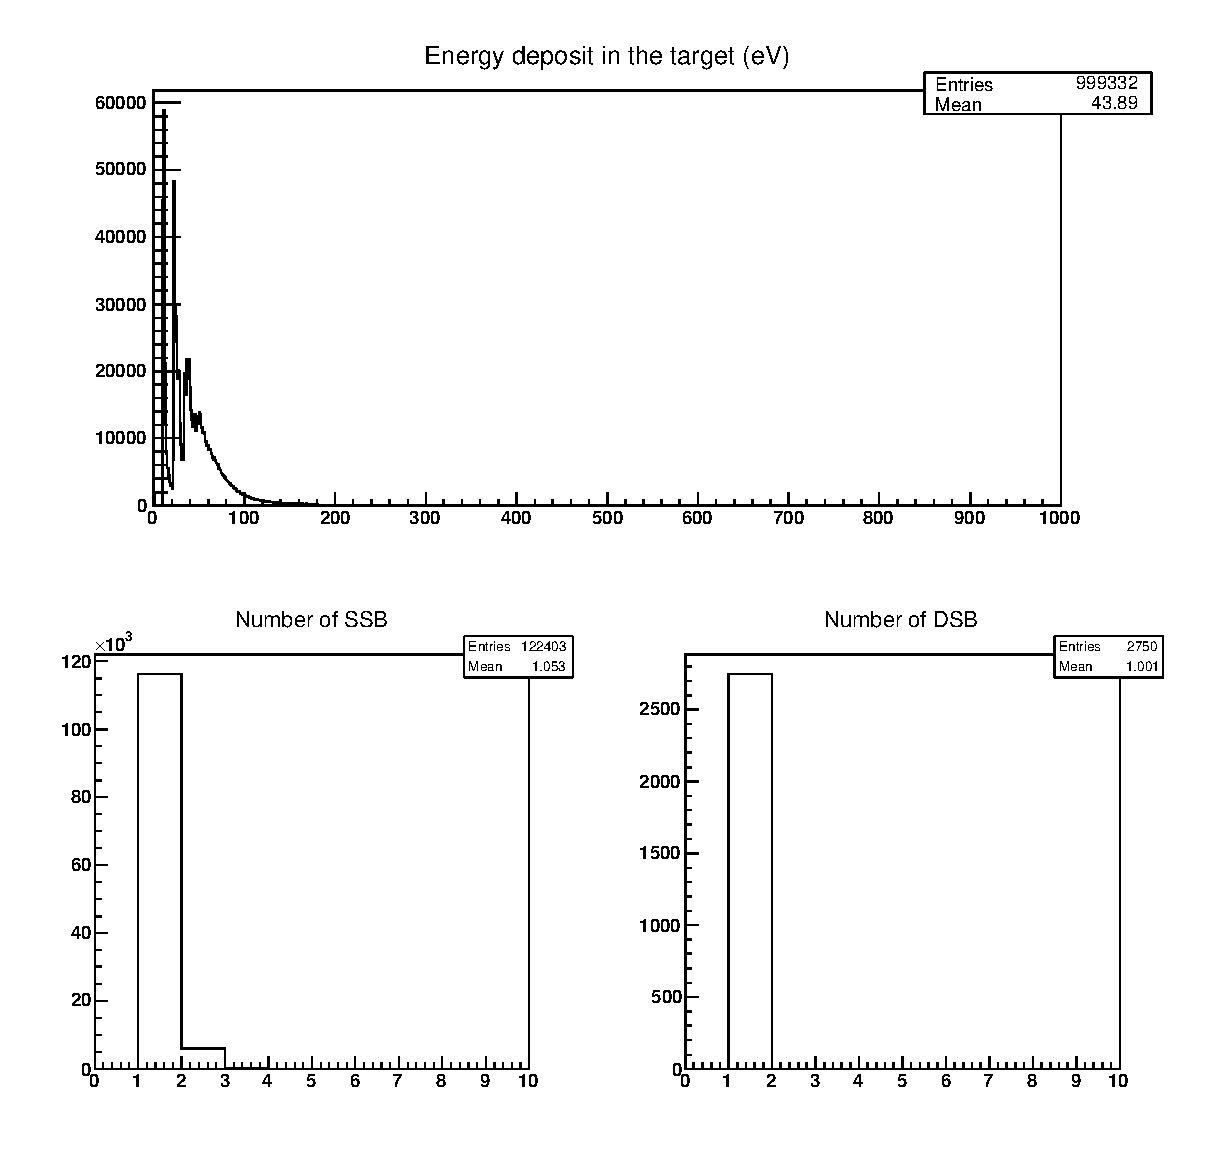
\includegraphics[width=.78\linewidth]{./Figures/1fzxp800ev.eps}
  \caption{800 eV}
  \label{fig:subi4}
\end{subfigure}
\begin{subfigure}{.5\textwidth}
  \centering
  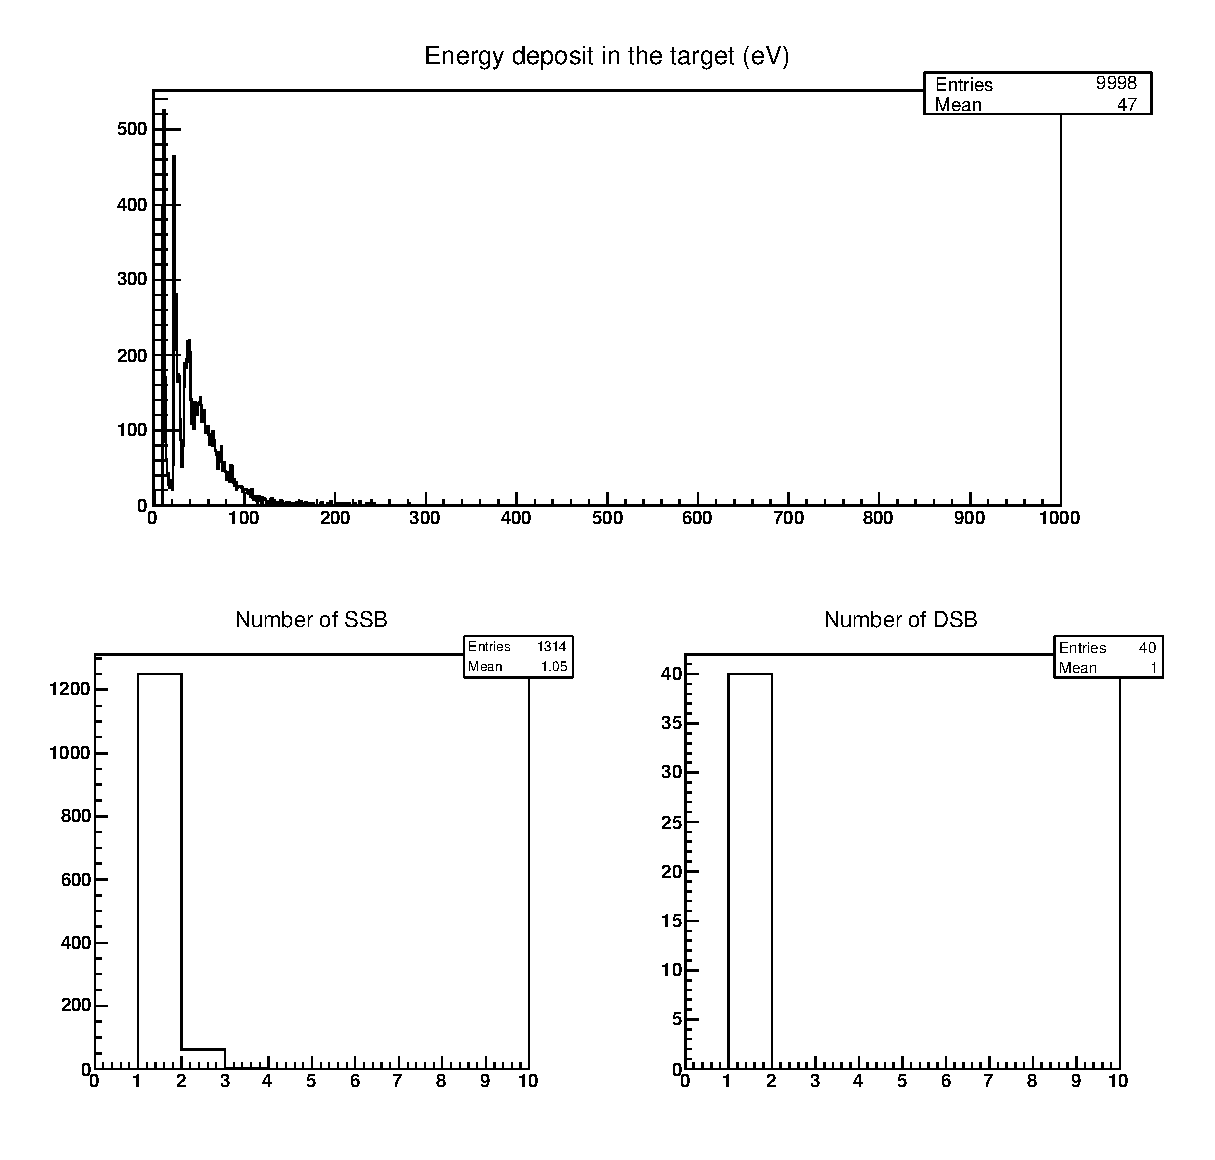
\includegraphics[width=.78\linewidth]{./Figures/1fzxp1kev.eps}
  \caption{1 keV}
  \label{fig:subi5}
\end{subfigure}%
\begin{subfigure}{.5\textwidth}
  \centering
  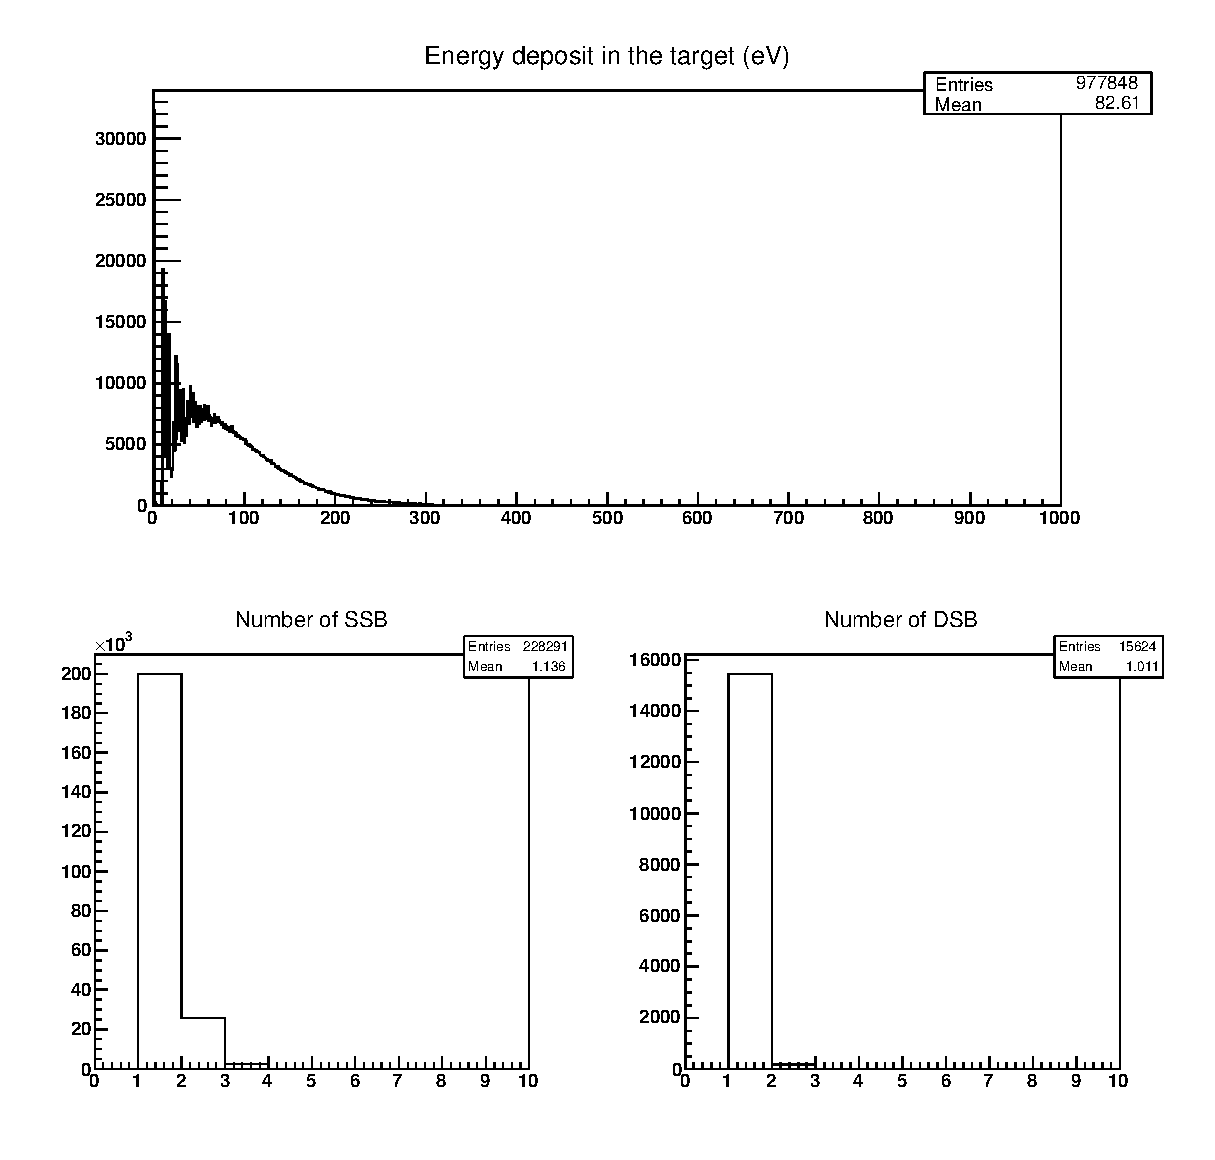
\includegraphics[width=.78\linewidth]{./Figures/1fzxp200kev.eps}
  \caption{200 keV}
  \label{fig:subi6}
\end{subfigure}
\begin{subfigure}{.5\textwidth}
  \centering
  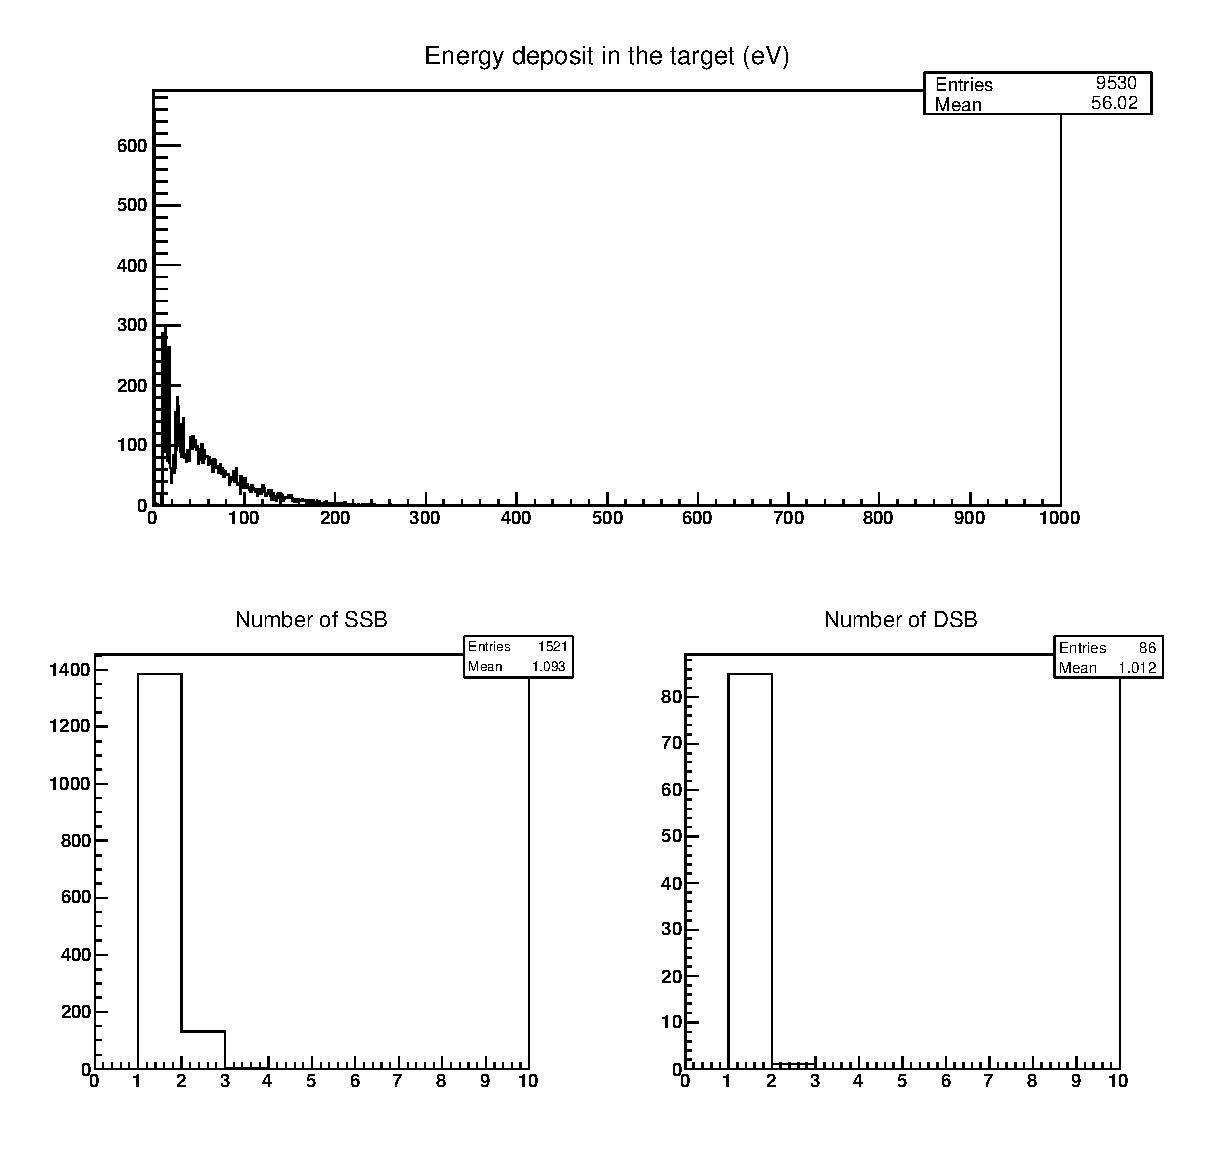
\includegraphics[width=.78\linewidth]{./Figures/1fzxp400kev.eps}
  \caption{400 keV}
  \label{fig:subi7}
\end{subfigure}%
\begin{subfigure}{.5\textwidth}
  \centering
  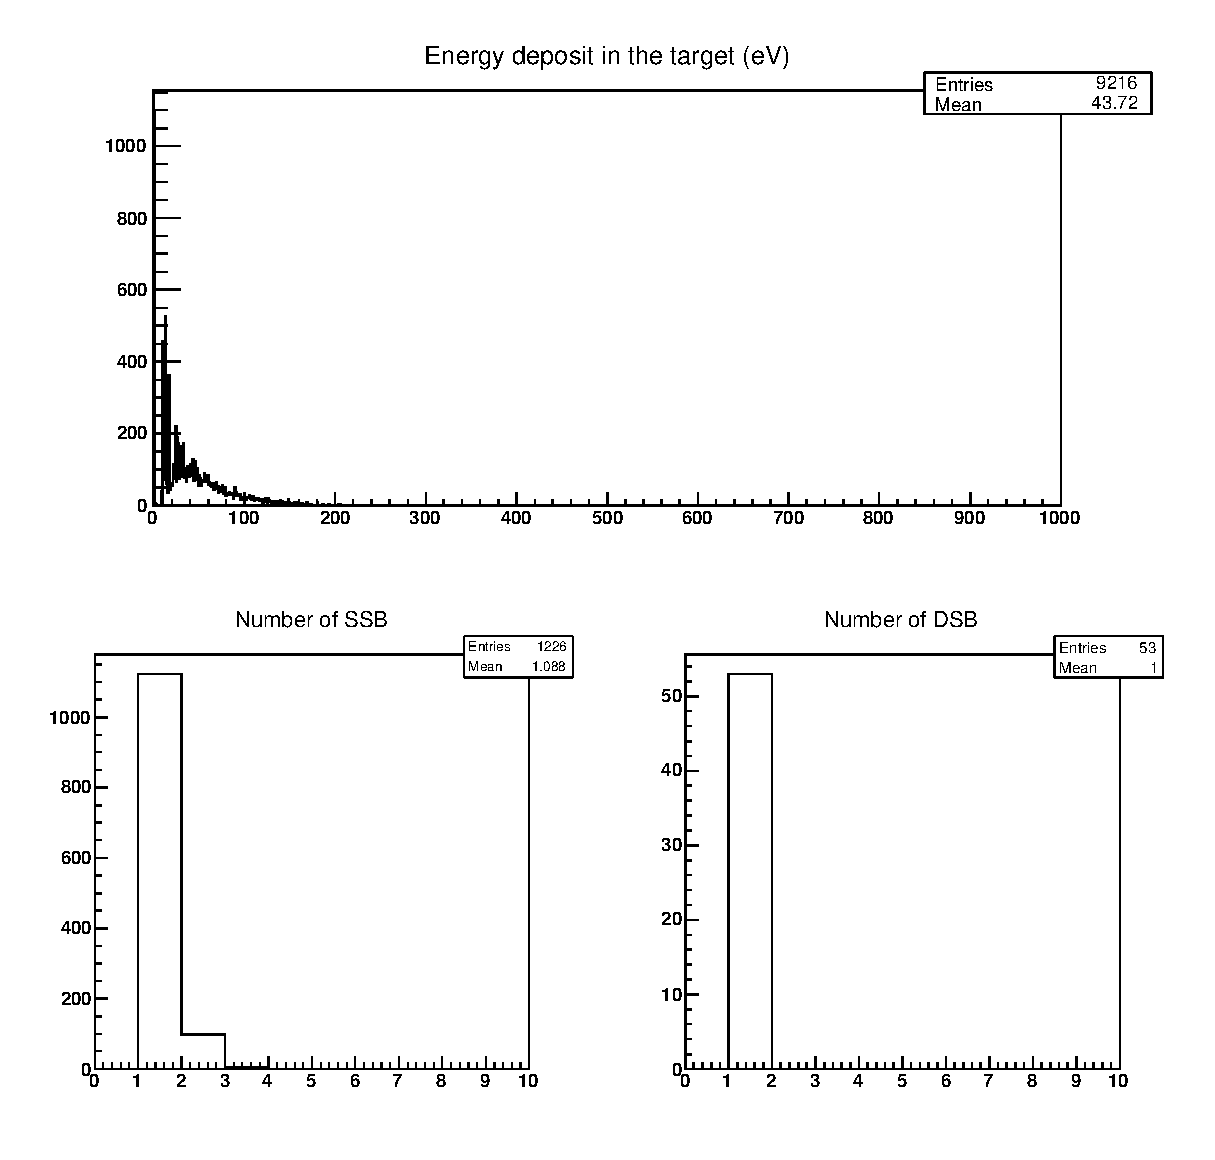
\includegraphics[width=.78\linewidth]{./Figures/1fzxp600kev.eps}
  \caption{600 keV}
  \label{fig:subi8}
\end{subfigure}
\caption{Rompimientos simples y dobles para 1FZX ($proton$)}
\label{fig:p2}
\end{figure}

Por otro lado se tienen las limitaciones de PDB4DNA, primero que nada tiene la restricción de como leer un archivo pdb, se basa en el uso del texto "TER" encontrando en estos archivos para leer cada cadena de ADN, el problema con esto radica en que no todos los archivos de este tipo contienen este comando, además de que por el momento este numero solo permite hacer uso de moléculas de ADN de dos cadenas y filtra el resto de la molécula para que no sea leída, esto nos podemos dar cuenta al comparar la figura de 1ZBB en Geant4(figura ~\ref{h}) y la vista en vmd(figura ~\ref{fig:1zbb}) como podemos observar la vista en Geant4 no tiene en cuenta los átomos que se encuentran al interior de los anillos de 1ZBB, a pesar de ser capaz de leer moléculas diferentes a las de ADN, muchas veces no muestra estas moléculas correctamente debido en parte a lectura del termino TER y a la selección de átomos que el programa realiza para formar los nucleótidos, aunque bien de modificarse correctamente se puede hacer posible la lectura y evaluación de estás moléculas.\\


Por ultimo PDB4DNA fue modificado de tal manera que en vez de hacer uso de las esferas ligadas a partir de baricentros hiciera uso de centros de masa, para esto se uso el archivo PDBlib, primero se definió la masa de los diferentes elementos (véase anexo ~\ref{app:M}),y luego se usaron las clases bases ya definidas en PDBlib para hacer los respectivos cálculos de centros de masa(véase anexo ~\ref{app:CM})), al hacer esto y visualizar en Geant4 no se nota ningún cambio alguno para ninguna de las dos moléculas (véase figuras ~\ref{fig:sub66} y ~\ref{fig:sub666}), también al realizar los eventos con los centros de masa y generar los debidos histogramas de deposición para ambas moléculas con las mismas energías observadas en la figuras ~\ref{fig:e},~\ref{fig:p},~\ref{fig:e2},~\ref{fig:p2}, no se presenta cambio alguno y debido a esto no se incluyeron, esto se puede deber a que la influencia de la magnitud del termino de la masa no afecta en mayor medida la posición de las partículas o el programa no esta tomando correctamente los nuevos baricentros, de cualquiera manera esto requiere más estudio debido a que la inclusión de centros de masa presenta un cambio relevante al modelo propuesto por pdb4dna con el uso de baricentros,  sin embargo al hacer histogramas de Root si es posible observar cambios respecto a las posiciones que de implementarse correctamente podrían alterar resultados en las deposiciones de energía en moléculas mucho más grandes y en consecuencia en los rompimientos dobles, los histogramas fueron realizados para cada cadena de ADN y su respectivas coordenadas x,y,z, para 1ZBB véase figuras: ~\ref{fig:canx},~\ref{fig:cany},~\ref{fig:canz}, y para 1FZX: ~\ref{fig:cax},~\ref{fig:cay},~\ref{fig:caz}.
\begin{figure}
\centering
\begin{subfigure}{.5\textwidth}
  \centering
  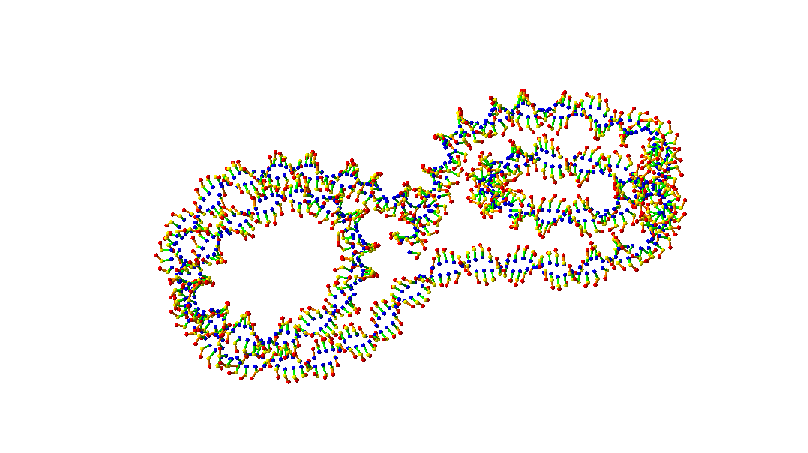
\includegraphics[width=.78\linewidth]{./Figures/baresi.png}
  \caption{Baricentro residuos }
  \label{fig:sub11}
\end{subfigure}%
\begin{subfigure}{.5\textwidth}
  \centering
  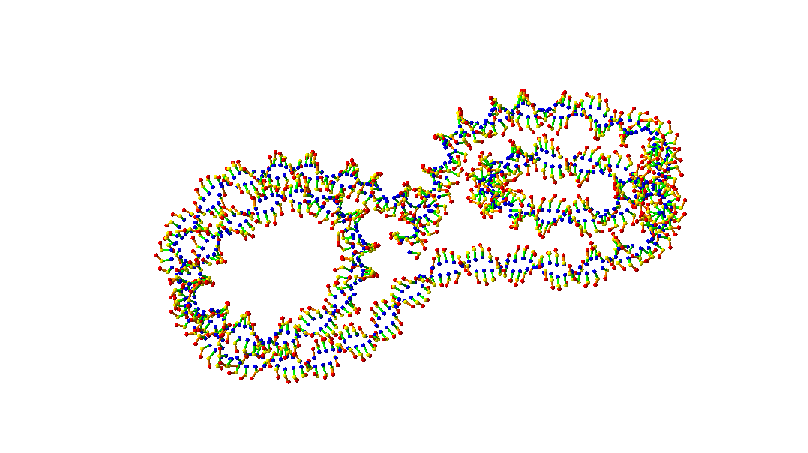
\includegraphics[width=.78\linewidth]{./Figures/baresi.png}
  \caption{Centros de masa residuos}
  \label{fig:sub22}
\end{subfigure}
\begin{subfigure}{.5\textwidth}
  \centering
  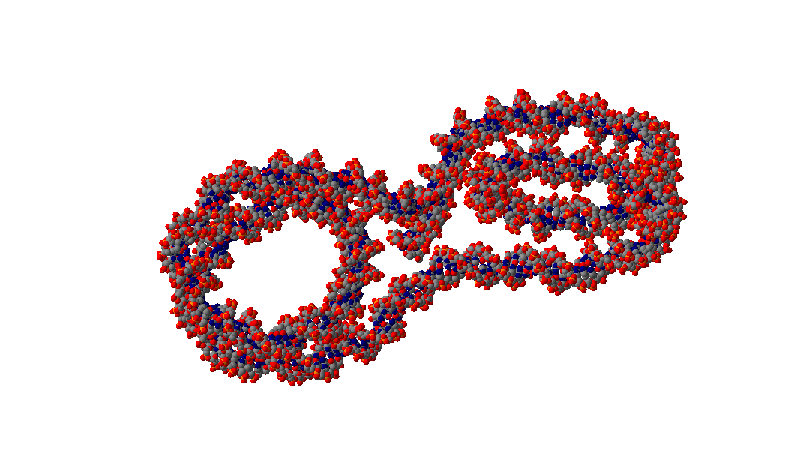
\includegraphics[width=.78\linewidth]{./Figures/bavdw.png}
  \caption{Baricentro VDW}
  \label{fig:sub33}
\end{subfigure}%
\begin{subfigure}{.5\textwidth}
  \centering
  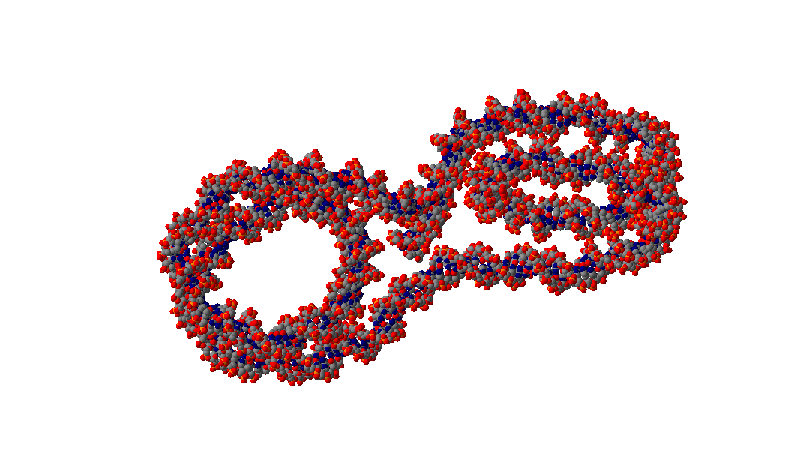
\includegraphics[width=.78\linewidth]{./Figures/bavdw.png}
  \caption{Centros de masa VDW}
  \label{fig:sub44}
\end{subfigure}
\begin{subfigure}{.5\textwidth}
  \centering
  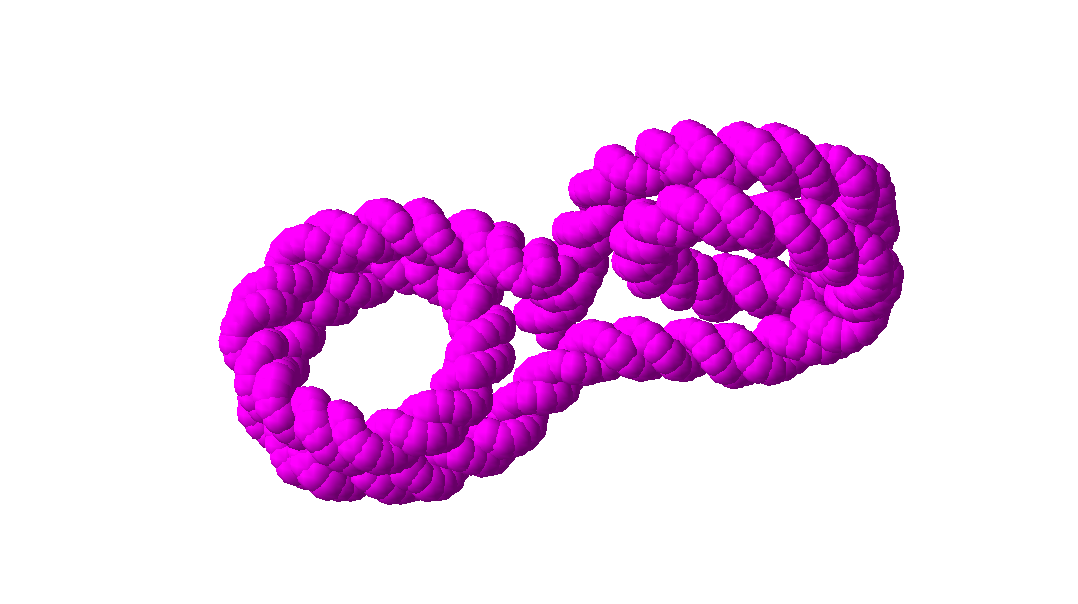
\includegraphics[width=.78\linewidth]{./Figures/a.png}
  \caption{Baricentro esferas ligadas}
  \label{fig:sub55}
\end{subfigure}%
\begin{subfigure}{.5\textwidth}
  \centering
  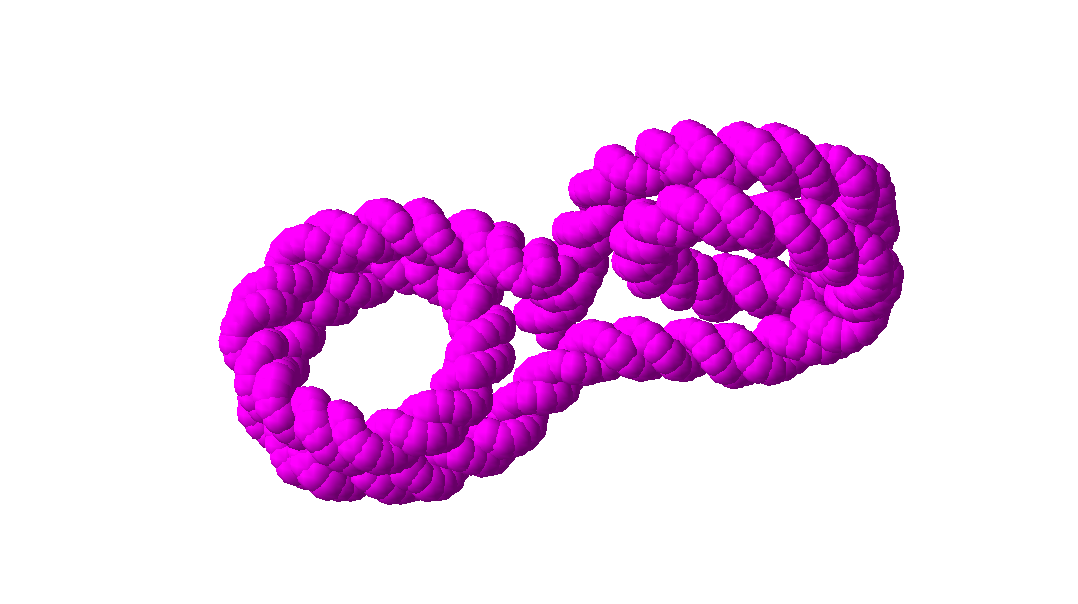
\includegraphics[width=.78\linewidth]{./Figures/a.png}
  \caption{Centros de masa esferas ligadas}
  \label{fig:sub66}
\end{subfigure}
\caption[Comparación de centros de masa y baricentros en Geant4 1ZBB]{Comparación representación centros de masa y baricentros en Geant4 para 1ZBB}
\label{h}
\end{figure}




\begin{figure}
\centering
\begin{subfigure}{.5\textwidth}
  \centering
  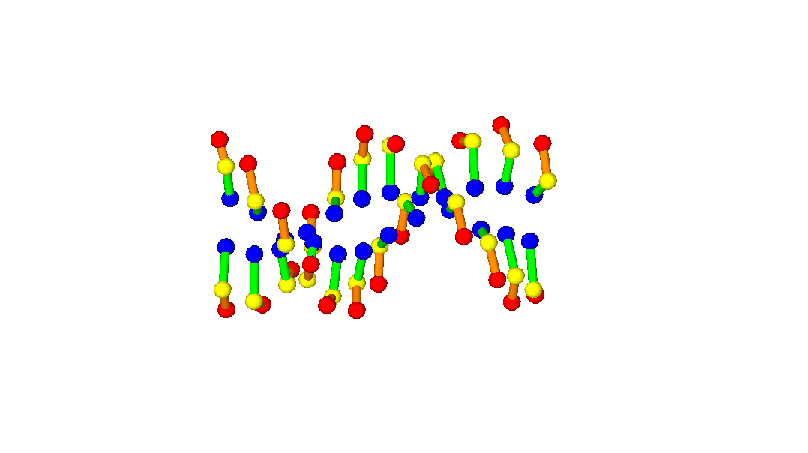
\includegraphics[width=.78\linewidth]{./Figures/1fzxresid.png}
  \caption{Baricentros residuos}
  \label{fig:sub111}
\end{subfigure}%
\begin{subfigure}{.5\textwidth}
  \centering
  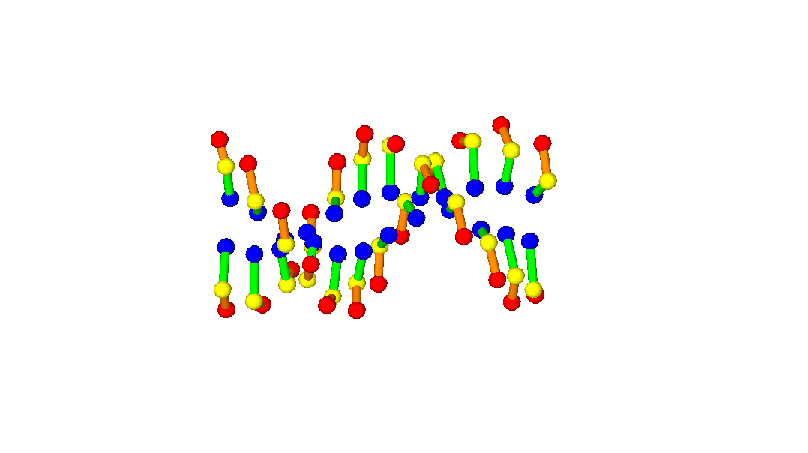
\includegraphics[width=.78\linewidth]{./Figures/1fzxresid.png}
  \caption{Centros de masa residuos}
  \label{fig:sub222}
\end{subfigure}
\begin{subfigure}{.5\textwidth}
  \centering
  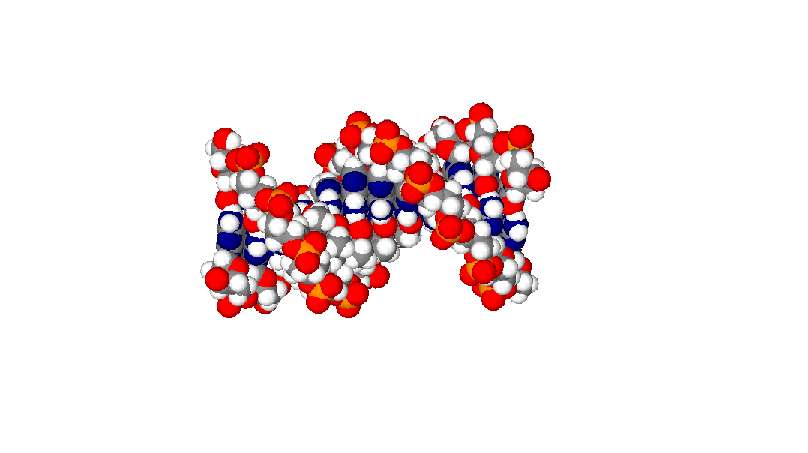
\includegraphics[width=.78\linewidth]{./Figures/1fzxvdw.png}
  \caption{Baricentro VDW}
  \label{fig:sub333}
\end{subfigure}%
\begin{subfigure}{.5\textwidth}
  \centering
  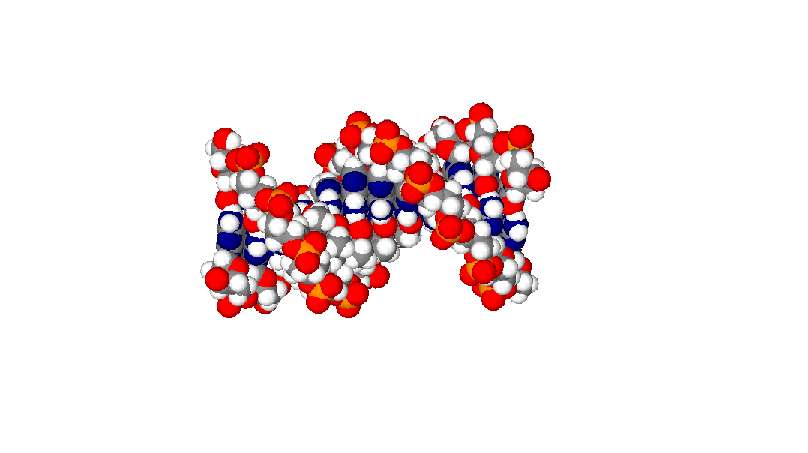
\includegraphics[width=.78\linewidth]{./Figures/1fzxvdw.png}
  \caption{Centros de masa VDW}
  \label{fig:sub444}
\end{subfigure}
\begin{subfigure}{.5\textwidth}
  \centering
  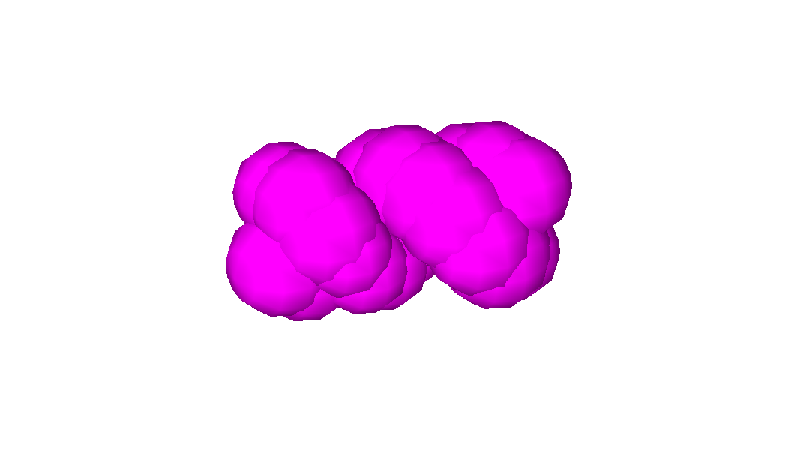
\includegraphics[width=.78\linewidth]{./Figures/1fzxba.png}
  \caption{Baricentro esferas ligadas}
  \label{fig:sub555}
\end{subfigure}%
\begin{subfigure}{.5\textwidth}
  \centering
  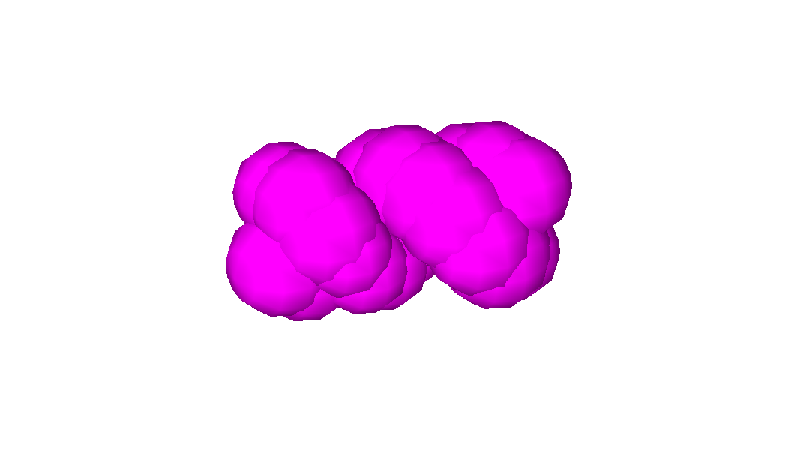
\includegraphics[width=.78\linewidth]{./Figures/1fzxba.png}
  \caption{Centros de masa esferas ligadas}
  \label{fig:sub666}
\end{subfigure}
\caption[Comparación de centros de masa y baricentros en Geant4 1FZX]{Comparación representación centros de masa y baricentros en Geant4 para 1FZX}
\label{hh}
\end{figure}




\begin{figure}[htbp]
    \centering
    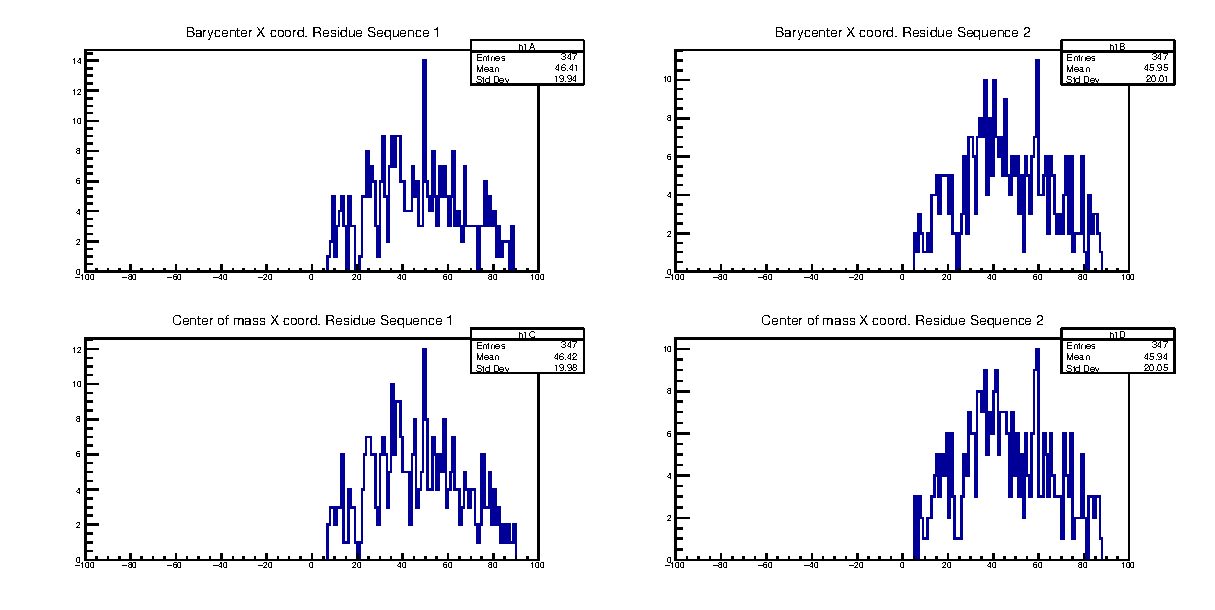
\includegraphics[width=1\linewidth]{./Figures/can1.eps}
  \caption[Baricentros en $x$ vs centros de masa en $x$ para 1ZBB]{Baricentros en $x$ vs centros de masa en $x$ para 1ZBB}
    \label{fig:canx}
\end{figure}

\begin{figure}[htbp]
    \centering
    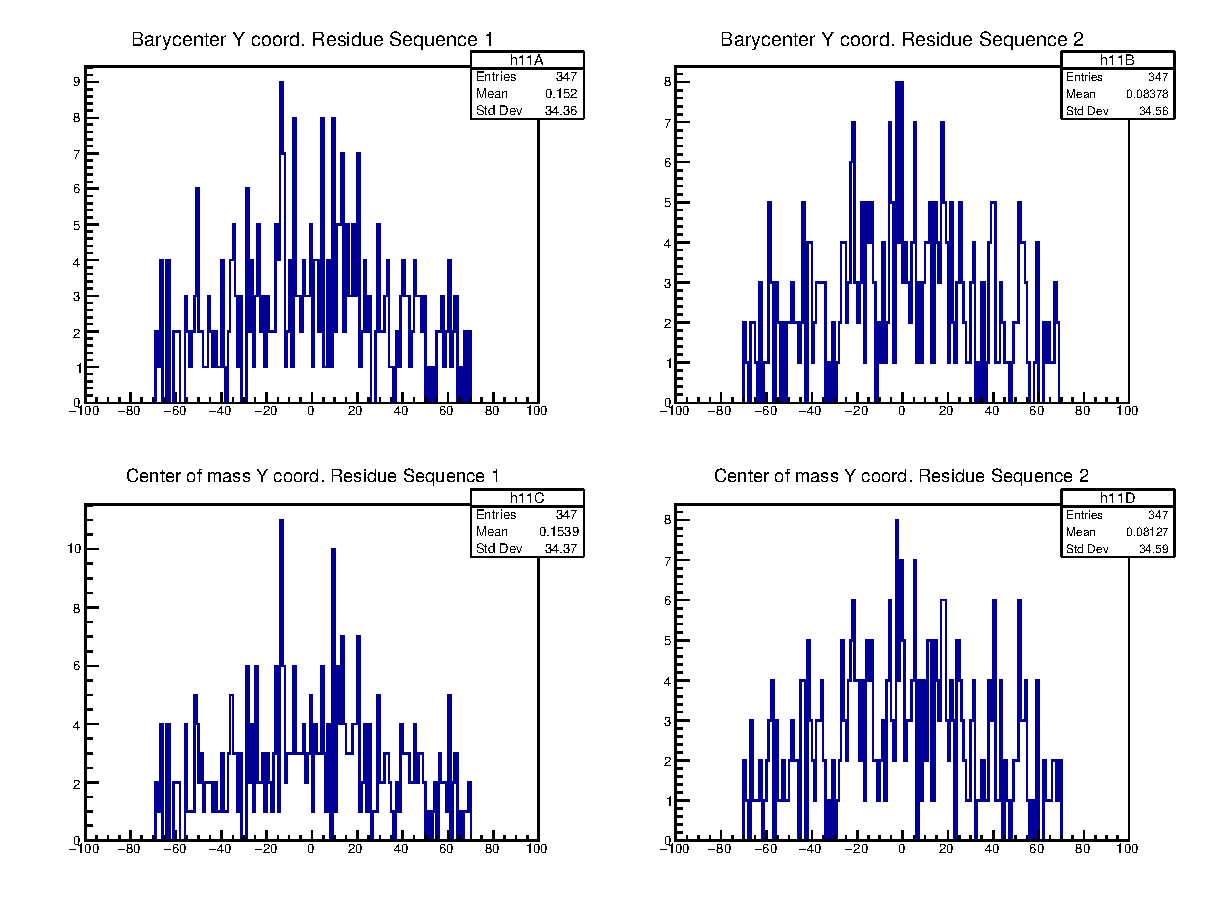
\includegraphics[width=1\linewidth]{./Figures/can2.eps}
    \caption[Baricentros en $y$ vs centros de masa en $y$ para 1ZBB]{Baricentros en $y$ vs centros de masa en $y$ para 1ZBB}
    \label{fig:cany}
\end{figure}

\begin{figure}[htbp]
    \centering
    \includegraphics[width=1\linewidth]{./Figures/can3.eps}
  \caption[Baricentros en $z$ vs centros de masa en $z$ para 1ZBB]{Baricentros en $z$ vs centros de masa en $z$ para 1ZBB}
    \label{fig:canz}
\end{figure}




\begin{figure}[htbp]
    \centering
    \includegraphics[width=1\linewidth]{./Figures/1fzx.eps}
  \caption[Baricentros en $x$ vs centros de masa en $x$ para 1FZX]{Baricentros en $x$ vs centros de masa en $x$ para 1FZX}
    \label{fig:cax}
\end{figure}

\begin{figure}[htbp]
    \centering
    \includegraphics[width=1\linewidth]{./Figures/1fzy.eps}
  \caption[Baricentros en $y$ vs centros de masa en $y$ para 1FZX]{Baricentros en $y$ vs centros de masa en $y$ para 1FZX}
    \label{fig:cay}
\end{figure}

\begin{figure}[htbp]
    \centering
    \includegraphics[width=1\linewidth]{./Figures/1fzz.eps}
  \caption[Baricentros en $z$ vs centros de masa en $z$ para 1FZX]{Baricentros en $z$ vs centros de masa en $z$ para 1FZX}
    \label{fig:caz}
\end{figure}
